         \chapter{Euclidian Geometry}
    \setcounter{figure}{1}
    \setcounter{subfigure}{1}
    \label{84e7e983e7dc2060d6909eddb5375c22}
          \section{Geometry Revision}
    \setcounter{figure}{1}
    \setcounter{subfigure}{1}
    \label{8eb3a75df362978731c03bbeab266515}
%          \section{ Points, lines and angles}
%     \nopagebreak
%             \label{m39370} $ \hspace{-5pt}\begin{array}{cccccccccccc}   
\includegraphics[width=0.75cm]{col11306.imgs/summary_fullmarks.png} &   
\includegraphics[width=0.75cm]{col11306.imgs/summary_video.png} &   \end{array} $ \hspace{2 pt}\raisebox{-5 pt}{} {(section shortcode: MG10087 )} \par 
%     
%     
%     
    \label{m39370*cid2}
            \subsection{ Introduction}
            \nopagebreak
      \label{m39370*id313235}The purpose of this section is to recap some of the ideas that you learned in geometry and trigonometry in earlier grades. You should feel comfortable with the work covered in this chapter before attempting to move onto the Grade 10 Geometry chapter\footnote{\raggedright{}"Geometry - Grade 10" <http://http://cnx.org/content/m32629/latest/>}, the Grade 10 Trigonometry chapter\footnote{\raggedright{}"Trigonometry - Grade 10" <http://http://cnx.org/content/m32620/latest/>} or the Grade 10 Analytical Geometry chapter\footnote{\raggedright{}"Analytical Geometry - Grade 10 [CAPS]" <http://http://cnx.org/content/m38370/latest/>}. This chapter revises:\par 
      \label{m39370*id313248}\begin{enumerate}[noitemsep, label=\textbf{\arabic*}. ] 
            \label{m39370*uid1}\item Terminology: vertices, sides, angles, parallel lines, perpendicular lines, diagonals, bisectors, transversals
\label{m39370*uid3}\item Properties of triangles
\label{m39370*uid4}\item Congruence
\label{m39370*uid5}\item Classification of angles into acute, right, obtuse, straight, reflex or revolution
\label{m39370*uid6}\item Theorem of Pythagoras which is used to calculate the lengths of sides of a right-angled triangle
\end{enumerate}
    \label{m39370*cid3}
            \subsection{ Points and Lines}
            \nopagebreak
      \label{m39370*id313683}The two simplest objects in geometry are \textsl{points} and \textsl{lines}.\par 
      \label{m39370*id313697}A point is a coordinate that marks a position in space (on a number line, on a plane or in three dimensions or even more) and is denoted by a dot. Points are usually labelled with a capital letter. Some examples of how points can be represented are shown in Figure~12.1.\par 
      \label{m39370*id313707}A line is a continuous set of coordinates in space and can be thought of as being formed when many points are placed next to each other. Lines can be straight or curved, but are always continuous. This means that there are never any breaks in the lines (if there are, they would be distinct lines denoted separately). The endpoints of lines are labeled with capital letters. Examples of two lines are shown in Figure~12.1.\par 
    \setcounter{subfigure}{0}
	\begin{figure}[H] % horizontal\label{m39370*uid7}
    \begin{center}
    \rule[.1in]{\figurerulewidth}{.005in} \\
        \label{m39370*uid7!!!underscore!!!media}\label{m39370*uid7!!!underscore!!!printimage}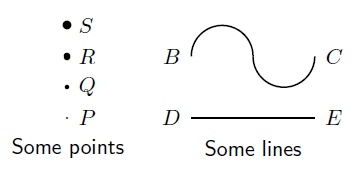
\includegraphics{col11306.imgs/m39370_MG10C13_001.png} % m39370;MG10C13\_001.png;;;6.0;8.5;
      \vspace{2pt}
    \vspace{\rubberspace}\par \begin{cnxcaption}
	  \small \textbf{Figure 12.1: }Examples of some points (labelled $P$, $Q$, $R$ and $S$\hspace{1ex}) and some lines (labelled $BC$ and $DE$\hspace{1ex}).
	\end{cnxcaption}
    \vspace{.1in}
    \rule[.1in]{\figurerulewidth}{.005in} \\
    \end{center}
 \end{figure}       
      \label{m39370*id313170}Lines are labelled according to the start point and end point. We call the line that starts at a point $A$ and ends at a point $B$, $AB$. Since the line from point $B$ to point $A$ is the same as the line from point $A$ to point $B$, we have that $AB=BA$.\par 
      \label{m39370*id313175}When there is no ambiguity (which is the case throughout this text) the length of the line between points $A$ and $B$ is also denoted $AB$\hspace{1ex}, the same as the notation to refer to the line itself. So if we say $AB=CD$\hspace{1ex} we mean that the length of the line between $A$ and $B$ is equal to the length of the line between $C$ and $D$.
\par 
      \label{m39370*eip-313}Note: in higher mathematics, where there might be some ambiguity between when we want refer to the length of the line and when we just want to refer to the line itself, the notation $|AB|$\hspace{1ex} is usually used to refer to the length of the line. In this case, if one says $|AB|=|CD|$, it means the lengths of the lines are the same, whereas if one says $AB=CD$, it means that the two lines actually coincide (i.e. they are the same). Throughout this text, however, this notation will not be used, and $AB=CD$ ALWAYS implies that the lengths are the same. \par \label{m39370*id314000}A line is measured in \textsl{units of length}. Some common units of length are listed in Table 12.1.\par 
    % \textbf{m39370*uid8}\par
          \begin{table}
    % \begin{t  \section{ Proofs and conjectures}
    \nopagebreak
            \label{m39352} $ \hspace{-5pt}\begin{array}{cccccccccccc}   
\includegraphics[width=0.75cm]{col11306.imgs/summary_fullmarks.png} &   \end{array} $ \hspace{2 pt}\raisebox{-5 pt}{} {(section shortcode: MG10094 )} \par 
    able}[H]
    % \\ '' '0'
        \begin{center}
      \label{m39370*uid8}
    \noindent
    \tabletail{%
        \hline
        \multicolumn{2}{|p{\mytableboxwidth}|}{\raggedleft \small \sl continued on next page}\\
        \hline
      }
      \tablelasttail{}
      \begin{xtabular}[t]{|l|l|}\hline
                \textbf{Unit of Length}
               &
                \textbf{Abbreviation}
              % make-rowspan-placeholders
     \tabularnewline\cline{1-1}\cline{2-2}
      %--------------------------------------------------------------------
        kilometre &
        km% make-rowspan-placeholders
     \tabularnewline\cline{1-1}\cline{2-2}
      %--------------------------------------------------------------------
        metre &
        m% make-rowspan-placeholders
     \tabularnewline\cline{1-1}\cline{2-2}
      %--------------------------------------------------------------------
        centimetre &
        cm% make-rowspan-placeholders
     \tabularnewline\cline{1-1}\cline{2-2}
      %--------------------------------------------------------------------
        millimetre &
        mm% make-rowspan-placeholders
     \tabularnewline\cline{1-1}\cline{2-2}
      %--------------------------------------------------------------------
    \end{xtabular}
      \end{center}
    \begin{center}{\small\bfseries Table 12.1}: Some common units of length and their abbreviations.\end{center}
    \begin{caption}{\small\bfseries Table 12.1}: Some common units of length and their abbreviations.\end{caption}
\end{table}
    \par
    \label{m39370*cid4}
            \subsection{ Angles}
            \nopagebreak
      \label{m39370*id314141}An \textsl{angle} is formed when two straight lines meet at a point. The point at which two lines meet is known as a \textsl{vertex}. Angles are labelled with a $\phantom{\rule{0.277778em}{0ex}}\hat{}\phantom{\rule{0.277778em}{0ex}}$ called a caret on a letter. For example, in Figure~12.2 the angle is at $\hat{B}$. Angles can also be labelled according to the line segments that make up the angle. For example, in Figure~12.2 the angle is made up when line segments $CB$ and $BA$ meet. So, the angle can be referred to as $\angle CBA$\hspace{1ex} or $\angle ABC$\hspace{1ex} or, if there is no ambiguity (i.e. there is only one angle at $B$) sometimes simply $\angle B$. The $\angle $ symbol is a short method of writing angle in geometry.\par 
      \label{m39370*id314241}Angles are measured in \textsl{degrees} which is denoted by ${}^{\circ }$, a small circle raised above the text in the same fashion as an exponent (or a superscript).\par 
      \label{m39370*eip-522}\label{m39370*notfhsst!!!underscore!!!id43812}
\begin{tabular}{cc}
	\hspace*{-50pt}\raisebox{-8 mm}{\hspace{-0.2in}
\includegraphics[width=0.75in]{col11306.imgs/psfact2.png} } & 
	\begin{minipage}{0.85\textwidth}
	\begin{note}
      {note: }
        \label{m39370*id316245335}Angles can also be measured in radians. At high school level you will only use degrees, but if you decide to take maths at university you will learn about radians.
        \par 
	\end{note}
	\end{minipage}
	\end{tabular}
	\par
      \par 
    \setcounter{subfigure}{0}
	\begin{figure}[H] % horizontal\label{m39370*uid9}
    \begin{center}
    \rule[.1in]{\figurerulewidth}{.005in} \\
        \label{m39370*uid9!!!underscore!!!media}\label{m39370*uid9!!!underscore!!!printimage}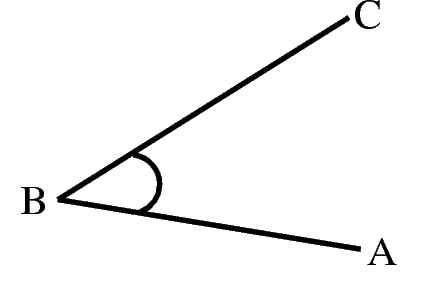
\includegraphics{col11306.imgs/m39370_MG10C13_002.png} % m39370;MG10C13\_002.png;;;6.0;8.5;
      \vspace{2pt}
    \vspace{\rubberspace}\par \begin{cnxcaption}
	  \small \textbf{Figure 12.2: }Angle labelled as $\hat{B}$, $\angle CBA$\hspace{1ex} or $\angle ABC$
	\end{cnxcaption}
    \vspace{.1in}
    \rule[.1in]{\figurerulewidth}{.005in} \\
    \end{center}
 \end{figure}       
    \setcounter{subfigure}{0}
	\begin{figure}[H] % horizontal\label{m39370*uid10}
    \begin{center}
    \rule[.1in]{\figurerulewidth}{.005in} \\
        \label{m39370*uid10!!!underscore!!!media}\label{m39370*uid10!!!underscore!!!printimage}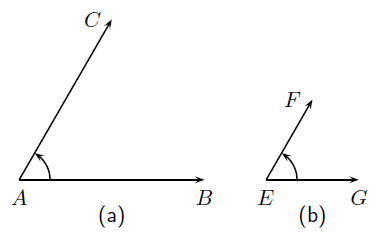
\includegraphics{col11306.imgs/m39370_MG10C13_003.png} % m39370;MG10C13\_003.png;;;6.0;8.5;
      \vspace{2pt}
    \vspace{\rubberspace}\par \begin{cnxcaption}
	  \small \textbf{Figure 12.3: }Examples of angles. $\hat{A}=\hat{E}$, even though the lines making up the angles are of different lengths.
	\end{cnxcaption}
    \vspace{.1in}
    \rule[.1in]{\figurerulewidth}{.005in} \\
    \end{center}
 \end{figure}       
      \label{m39370*uid11}
            \subsubsection{ Measuring angles}
            \nopagebreak
        \label{m39370*id314363}The size of an angle does not depend on the length of the lines that are joined to make up the angle, but depends only on how both the lines are placed as can be seen in Figure~12.3. This means that the idea of length cannot be used to measure angles. An angle is a rotation around the vertex.\par 
        \label{m39370*uid12}
            \subsubsection{ Using a Protractor}
            \nopagebreak
          \label{m39370*id314383}A protractor is a simple tool that is used to measure angles. A picture of a protractor is shown in Figure~12.4.\par 
    \setcounter{subfigure}{0}
	\begin{figure}[H] % horizontal\label{m39370*uid13}
    \begin{center}
    \rule[.1in]{\figurerulewidth}{.005in} \\
        \label{m39370*uid13!!!underscore!!!media}\label{m39370*uid13!!!underscore!!!printimage}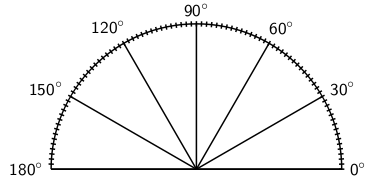
\includegraphics{col11306.imgs/m39370_MG10C13_004.png} % m39370;MG10C13\_004.png;;;6.0;8.5;
      \vspace{2pt}
    \vspace{\rubberspace}\par \begin{cnxcaption}
	  \small \textbf{Figure 12.4: }Diagram of a protractor.
	\end{cnxcaption}
    \vspace{.1in}
    \rule[.1in]{\figurerulewidth}{.005in} \\
    \end{center}
 \end{figure}       
          \label{m39370*id314404}
            \textbf{Method:}
          \par 
          \label{m39370*id314412}Using a protractor\par 
          \label{m39370*id314417}\begin{enumerate}[noitemsep, label=\textbf{\arabic*}. ] 
            \label{m39370*uid14}\item Place the bottom line of the protractor along one line of the angle so that the other line of the angle points at the degree markings.
\label{m39370*uid15}\item Move the protractor along the line so that the centre point on the protractor is at the vertex of the two lines that make up the angle.
\label{m39370*uid16}\item Follow the second line until it meets the marking on the protractor and read off the angle. Make sure you start measuring at 0${}^{\circ }$.
\end{enumerate}
\label{m39370*secfhsst!!!underscore!!!id175}
            \subsubsection{  Measuring Angles : Use a protractor to measure the following angles:}
            \nopagebreak
          \label{m39370*id314481}
    \setcounter{subfigure}{0}
	\begin{figure}[H] % horizontal\label{m39370*id314484}
    \begin{center}
    \label{m39370*id314484!!!underscore!!!media}\label{m39370*id314484!!!underscore!!!printimage}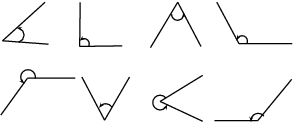
\includegraphics{col11306.imgs/m39370_MG10C13_005.png} % m39370;MG10C13\_005.png;;;6.0;8.5;
      \vspace{2pt}
    \vspace{.1in}
    \end{center}
 \end{figure}       
          \par 
      \label{m39370*uid17}
            \subsubsection{ Special Angles}
            \nopagebreak
        \label{m39370*id314513}What is the smallest angle that can be drawn? The figure below shows two lines ($CA$ and $AB$) making an angle at a common vertex $A$. If line $CA$ is rotated around the common vertex $A$, down towards line $AB$, then the smallest angle that can be drawn occurs when the two lines are pointing in the same direction. This gives an angle of 0${}^{\circ }$. This is shown in Figure~12.6\par 
        \label{m39370*id314590}
    \setcounter{subfigure}{0}
	\begin{figure}[H] % horizontal\label{m39370*id314593}
    \begin{center}
    \label{m39370*id314593!!!underscore!!!media}\label{m39370*id314593!!!underscore!!!printimage}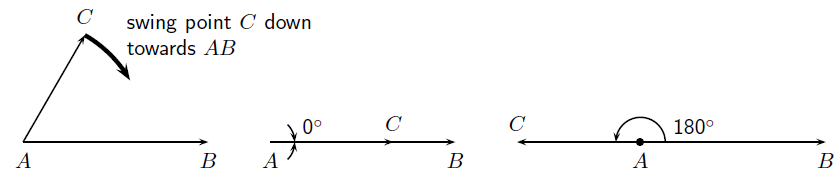
\includegraphics[width=.8\columnwidth]{col11306.imgs/m39370_MG10C13_006.png} % m39370;MG10C13\_006.png;;;6.0;8.5;
      \vspace{2pt}
    \vspace{.1in}
    \end{center}
 \end{figure}       
        \par 
        \label{m39370*id314599}If line $CA$ is now swung upwards, any other angle can be obtained. If line $CA$ and line $AB$ point in opposite directions (the third case in Figure~12.6) then this forms an angle of 180${}^{\circ }$.\par 
\label{m39370*notfhsst!!!underscore!!!id201}
\begin{tabular}{cc}
	   \hspace*{-50pt}\raisebox{-8 mm}{ 
\includegraphics[width=0.5in]{col11306.imgs/pstip2.png}  }& 
	\begin{minipage}{0.85\textwidth}
	\begin{note}
      {tip: }If three points $A$, $B$ and $C$ lie on a straight line, then the angle between them is 180${}^{\circ }$. Conversely, if the angle between three points is 180${}^{\circ }$, then the points lie on a straight line.
	\end{note}
	\end{minipage}
	\end{tabular}
	\par
        \label{m39370*id314704}An angle of 90${}^{\circ }$ is called a \textsl{right angle}. A right angle is half the size of the angle made by a straight line (180${}^{\circ }$). We say $CA$ is \textsl{perpendicular} to $AB$ or $CA\perp AB$\hspace{1ex}. An angle twice the size of a straight line is 360${}^{\circ }$. An angle measuring 360${}^{\circ }$ looks identical to an angle of 0${}^{\circ }$, except for the labelling. We call this a \textsl{revolution}.\par 
    \setcounter{subfigure}{0}
	\begin{figure}[H] % horizontal\label{m39370*uid18}
    \begin{center}
    \rule[.1in]{\figurerulewidth}{.005in} \\
        \label{m39370*uid18!!!underscore!!!media}\label{m39370*uid18!!!underscore!!!printimage}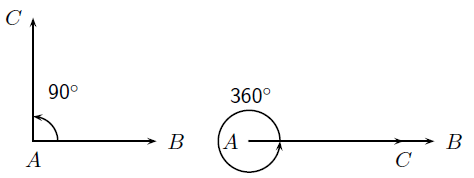
\includegraphics[width=.8\columnwidth]{col11306.imgs/m39370_MG10C13_007.png} % m39370;MG10C13\_007.png;;;6.0;8.5;
      \vspace{2pt}
    \vspace{\rubberspace}\par \begin{cnxcaption}
	  \small \textbf{Figure 12.7: }An angle of 90${}^{\circ }$ is known as a \textsl{right angle}.
	\end{cnxcaption}
    \vspace{.1in}
    \rule[.1in]{\figurerulewidth}{.005in} \\
    \end{center}
 \end{figure}       
\label{m39370*secfhsst!!!underscore!!!id210}
            \subsubsection{  Angles larger than 360${}^{\circ }$ }
            \nopagebreak
        \label{m39370*id314877}All angles larger than 360${}^{\circ }$ also look like we have seen them before. If you are given an angle that is larger than 360${}^{\circ }$, continue subtracting 360${}^{\circ }$ from the angle, until you get an answer that is between 0${}^{\circ }$and 360${}^{\circ }$. Angles that measure more than 360${}^{\circ }$ are largely for mathematical convenience. \par 
\label{m39370*notfhsst!!!underscore!!!id213}
\begin{tabular}{cc}
	   \hspace*{-50pt}\raisebox{-8 mm}{ 
\includegraphics[width=0.5in]{col11306.imgs/pstip2.png}  }& 
	\begin{minipage}{0.85\textwidth}
	\begin{note}
      {tip: }
        \label{m39370*id314971}\begin{itemize}[noitemsep]
            \label{m39370*uid19}\item \textsl{Acute angle}: An angle $\ge {0}^{\circ }$ and $\lessthan{}{90}^{\circ }$.
\label{m39370*uid20}\item \textsl{Right angle}: An angle measuring ${90}^{\circ }$.
\label{m39370*uid21}\item \textsl{Obtuse angle}: An angle $\greatthan{}{90}^{\circ }$ and $\lessthan{}{180}^{\circ }$.
\label{m39370*uid22}\item \textsl{Straight angle}: An angle measuring 180${}^{\circ }$.
\label{m39370*uid23}\item \textsl{Reflex angle}: An angle $\greatthan{}{180}^{\circ }$ and $\lessthan{}{360}^{\circ }$.
\label{m39370*uid24}\item \textsl{Revolution}: An angle measuring ${360}^{\circ }$.
\end{itemize}
        \label{m39370*id315224}These are simply labels for angles in particular ranges, shown in Figure~12.8.\par 
	\end{note}
	\end{minipage}
	\end{tabular}
	\par
    \setcounter{subfigure}{0}
	\begin{figure}[H] % horizontal\label{m39370*uid25}
    \begin{center}
    \rule[.1in]{\figurerulewidth}{.005in} \\
        \label{m39370*uid25!!!underscore!!!media}\label{m39370*uid25!!!underscore!!!printimage}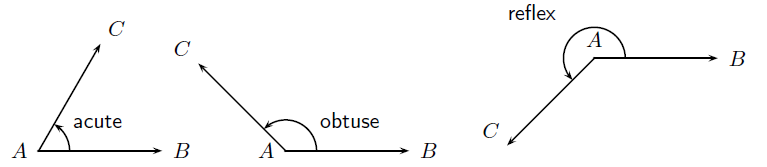
\includegraphics[width=.8\columnwidth]{col11306.imgs/m39370_MG10C13_008.png} % m39370;MG10C13\_008.png;;;6.0;8.5;
      \vspace{2pt}
    \vspace{\rubberspace}\par \begin{cnxcaption}
	  \small \textbf{Figure 12.8: }Three types of angles defined according to their ranges.
	\end{cnxcaption}
    \vspace{.1in}
    \rule[.1in]{\figurerulewidth}{.005in} \\
    \end{center}
 \end{figure}       
        \label{m39370*id315245}Once angles can be measured, they can then be compared. For example, all right angles are 90${}^{\circ }$, therefore all right angles are equal and an obtuse angle will always be larger than an acute angle.\par \label{m39370*eip-752}The following video summarizes what you have learnt so far about angles.
    \setcounter{subfigure}{0}
	\begin{figure}[H] % horizontal\label{m39370*angles-1}
    \textnormal{Khan Academy video on angles - 1}\vspace{.1in} \nopagebreak
  \label{m39370*yt-media1}\label{m39370*yt-video1}
            \raisebox{-5 pt}{ 
\includegraphics[width=0.5cm]{col11306.imgs/summary_www.png}} { (Video:  MG10088 )}
      \vspace{2pt}
    \vspace{.1in}
 \end{figure}       
Note that for high school trigonometry you will be using degrees, not radians as stated in the video. \par 
      \label{m39370*uid26}
            \subsubsection{ Special Angle Pairs}
            \nopagebreak
        \label{m39370*id315274}In Figure~12.10, straight lines $AB$ and $CD$ intersect at point X, forming four angles: $\hat{{X}_{1}}$ or $\angle BXD$\hspace{1ex}, $\hat{{X}_{2}}$\hspace{1ex} or $\angle BXC$\hspace{1ex}, $\hat{{X}_{3}}$\hspace{1ex} or $\angle CXA$\hspace{1ex} and $\hat{{X}_{4}}$\hspace{1ex} or $\angle AXD$\hspace{1ex}.\par 
    \setcounter{subfigure}{0}
	\begin{figure}[H] % horizontal\label{m39370*uid27}
    \begin{center}
    \rule[.1in]{\figurerulewidth}{.005in} \\
        \label{m39370*uid27!!!underscore!!!media}\label{m39370*uid27!!!underscore!!!printimage}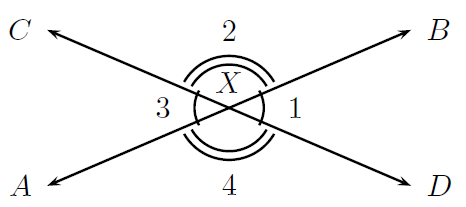
\includegraphics[width=.5\columnwidth]{col11306.imgs/m39370_MG10C13_009.png} % m39370;MG10C13\_009.png;;;6.0;8.5;
      \vspace{2pt}
    \vspace{\rubberspace}\par \begin{cnxcaption}
	  \small \textbf{Figure 12.10: }Two intersecting straight lines with vertical angles $\hat{{X}_{1}},\hat{{X}_{3}}$ and $\hat{{X}_{2}},\hat{{X}_{4}}$.
	\end{cnxcaption}
    \vspace{.1in}
    \rule[.1in]{\figurerulewidth}{.005in} \\
    \end{center}
 \end{figure}       
        \label{m39370*id315545}The table summarises the special angle pairs that result.\par 
    % \textbf{m39370*id315548}\par
          \begin{table}
    % \begin{table}[H]
    % \\ '' '0'
        \begin{center}
      \label{m39370*id315548}
    \noindent
    \tabletail{%
        \hline
        \multicolumn{3}{|p{\mytableboxwidth}|}{\raggedleft \small \sl continued on next page}\\
        \hline
      }
      \tablelasttail{}
      \begin{xtabular}[t]{|l|l|l|}\hline
        Special Angle &
        Property &
        Example% make-rowspan-placeholders
     \tabularnewline\cline{1-1}\cline{2-2}\cline{3-3}
      %--------------------------------------------------------------------
        adjacent angles &
        share a common vertex and a common side &
        $\left(\hat{{X}_{1}},\hat{{X}_{2}}\right)$, $\left(\hat{{X}_{2}},\hat{{X}_{3}}\right)$, $\left(\hat{{X}_{3}},\hat{{X}_{4}}\right)$, $\left(\hat{{X}_{4}},\hat{{X}_{1}}\right)$% make-rowspan-placeholders
     \tabularnewline\cline{1-1}\cline{2-2}\cline{3-3}
      %--------------------------------------------------------------------
        linear pair (adjacent angles on a straight line) &
        adjacent angles formed by two intersecting straight lines that by definition add to 180${}^{\circ }$ &
                  $\hat{{X}_{1}}+\hat{{X}_{2}}={180}^{\circ }$;
                  $\hat{{X}_{2}}+\hat{{X}_{3}}={180}^{\circ }$;
                  $\hat{{X}_{3}}+\hat{{X}_{4}}={180}^{\circ }$;
                  $\hat{{X}_{4}}+\hat{{X}_{1}}={180}^{\circ }$
                % make-rowspan-placeholders
     \tabularnewline\cline{1-1}\cline{2-2}\cline{3-3}
      %--------------------------------------------------------------------
        opposite angles &
        angles formed by two intersecting straight lines that share a vertex but do not share any sides &
                  $\hat{{X}_{1}}=\hat{{X}_{3}}$;
                  $\hat{{X}_{2}}=\hat{{X}_{4}}$
                % make-rowspan-placeholders
     \tabularnewline\cline{1-1}\cline{2-2}\cline{3-3}
      %--------------------------------------------------------------------
        supplementary angles &
      % My position: 1
    % my spanname: 
    % my ct of spanspec: 0
    % my column-count: 2
    \multicolumn{2}{c|}{two angles whose sum is 180${}^{\circ }$}
     \tabularnewline\cline{1-1}\cline{2-2}\cline{3-3}
      %--------------------------------------------------------------------
        complementary angles &
      % My position: 1
    % my spanname: 
    % my ct of spanspec: 0
    % my column-count: 2
    \multicolumn{2}{c|}{two angles whose sum is 90${}^{\circ }$}
     \tabularnewline\cline{1-1}\cline{2-2}\cline{3-3}
      %--------------------------------------------------------------------
    \end{xtabular}
      \end{center}
    \begin{center}{\small\bfseries Table 12.2}\end{center}
    \begin{caption}{\small\bfseries Table 12.2}\end{caption}
\end{table}
    \par
\label{m39370*notfhsst!!!underscore!!!id423}
\begin{tabular}{cc}
	   \hspace*{-50pt}\raisebox{-8 mm}{ 
\includegraphics[width=0.5in]{col11306.imgs/pstip2.png}  }& 
	\begin{minipage}{0.85\textwidth}
	\begin{note}
      {tip: }The opposite angles formed by the intersection of two straight lines are equal. Adjacent angles on a straight line are supplementary.
	\end{note}
	\end{minipage}
	\end{tabular}
	\par
      \label{m39370*eip-433}The following video summarises what you have learnt so far
    \setcounter{subfigure}{0}
	\begin{figure}[H] % horizontal\label{m39370*angles-2}
    \textnormal{Khan Academy video on angles - 2}\vspace{.1in} \nopagebreak
  \label{m39370*yt-media2}\label{m39370*yt-video2}
            \raisebox{-5 pt}{ 
\includegraphics[width=0.5cm]{col11306.imgs/summary_www.png}} { (Video:  MG10089 )}
      \vspace{2pt}
    \vspace{.1in}
 \end{figure}       \par 
      \label{m39370*uid28}
            \subsubsection{ Parallel Lines intersected by Transversal Lines}
            \nopagebreak
            \label{m39370*id316211}Two lines intersect if they cross each other at a point. For example, at a traffic intersection two or more streets intersect; the middle of the intersection is the common point between the streets.\par 
        \label{m39370*id316216}\textsl{Parallel lines} are lines that never intersect. For example the tracks of a railway line are parallel (for convenience, sometimes mathematicians say they intersect at 'a point at infinity', i.e. an infinite distance away). We wouldn't want the tracks to intersect after as that would be catastrophic for the train!\par 
        \label{m39370*id316225}
    \setcounter{subfigure}{0}
	\begin{figure}[H] % horizontal\label{m39370*id316228}
    \begin{center}
    \label{m39370*id316228!!!underscore!!!media}\label{m39370*id316228!!!underscore!!!printimage}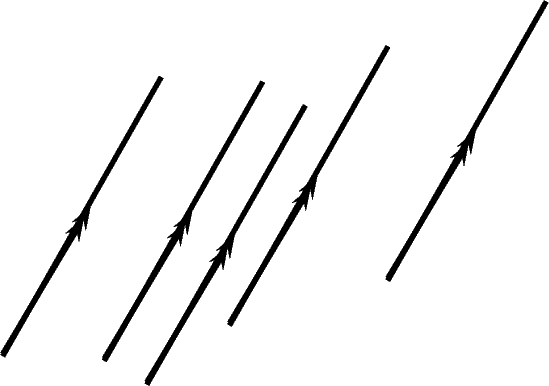
\includegraphics{col11306.imgs/m39370_MG10C13_010.png} % m39370;MG10C13\_010.png;;;6.0;8.5;
      \vspace{2pt}
    \vspace{.1in}
    \end{center}
 \end{figure}       
        \par 
        \label{m39370*id316235}All these lines are parallel to each other. Notice the pair of arrow symbols for parallel.\par 
\label{m39370*notfhsst!!!underscore!!!id438}
\begin{tabular}{cc}
	\hspace*{-50pt}\raisebox{-8 mm}{\hspace{-0.2in}
\includegraphics[width=0.75in]{col11306.imgs/psfact2.png} } & 
	\begin{minipage}{0.85\textwidth}
	\begin{note}
      {note: }
        \label{m39370*id316245}A section of the Australian National Railways Trans-Australian line is perhaps one of the longest pairs of man-made parallel lines.\par 
        \label{m39370*id316258}
          \label{m39370*id316258!!!underscore!!!quote}\begin{quote}{\sl \textbf{Longest Railroad Straight} (Source: www.guinnessworldrecords.com)
The Australian National Railways Trans-Australian line over the Nullarbor Plain, is 478~km (297 miles) dead straight, from Mile 496, between Nurina and Loongana, Western Australia, to Mile 793, between Ooldea and Watson, South Australia.} % end \textsl
    \end{quote}
        \par 
	\end{note}
	\end{minipage}
	\end{tabular}
	\par
        \label{m39370*id316273}A \textsl{transversal} of two or more lines is a line that intersects these lines. For example in Figure~12.13, $AB$ and $CD$ are two parallel lines and $EF$ is a transversal. We say $AB\parallel CD$. The properties of the angles formed by these intersecting lines are summarised in the table below.\par 
    \setcounter{subfigure}{0}
	\begin{figure}[H] % horizontal\label{m39370*uid29}
    \begin{center}
    \rule[.1in]{\figurerulewidth}{.005in} \\
        \label{m39370*uid29!!!underscore!!!media}\label{m39370*uid29!!!underscore!!!printimage}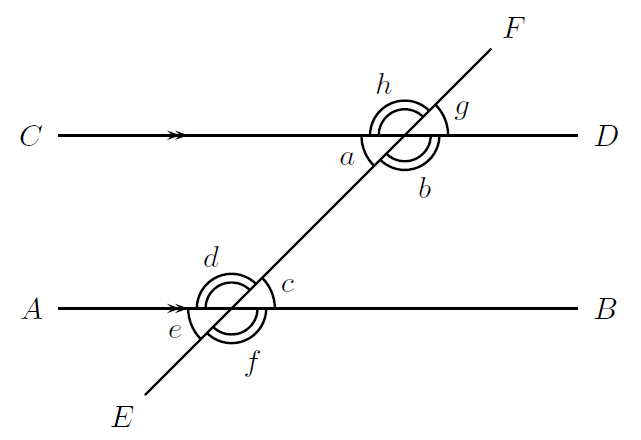
\includegraphics[width=.8\columnwidth]{col11306.imgs/m39370_MG10C13_011.png} % m39370;MG10C13\_011.png;;;6.0;8.5;
      \vspace{2pt}
    \vspace{\rubberspace}\par \begin{cnxcaption}
	  \small \textbf{Figure 12.13: }Parallel lines intersected by a transversal
	\end{cnxcaption}
    \vspace{.1in}
    \rule[.1in]{\figurerulewidth}{.005in} \\
    \end{center}
 \end{figure}       
    % \textbf{m39370*uid30}\par
          \begin{table}
    % \begin{table}[H]
    % \\ '' '0'
        \begin{center}
      \label{m39368*uid92}
    \noindent
    \tabletail{%
        \hline
        \multicolumn{2}{|p{\mytableboxwidth}|}{\raggedleft \small \sl continued on next page}\\
        \hline
      }
      \tablelasttail{}
      \begin{xtabular}[t]{|l|l|}\hline
        Sides &
        Name% make-rowspan-placeholders
     \tabularnewline\cline{1-1}\cline{2-2}
      %--------------------------------------------------------------------
        5 &
        pentagon% make-rowspan-placeholders
     \tabularnewline\cline{1-1}\cline{2-2}
      %--------------------------------------------------------------------
        6 &
        hexagon% make-rowspan-placeholders
     \tabularnewline\cline{1-1}\cline{2-2}
      %--------------------------------------------------------------------
        7 &
        heptagon% make-rowspan-placeholders
     \tabularnewline\cline{1-1}\cline{2-2}
      %--------------------------------------------------------------------
        8 &
        octagon% make-rowspan-placeholders
     \tabularnewline\cline{1-1}\cline{2-2}
      %--------------------------------------------------------------------
        10 &
        decagon% make-rowspan-placeholders
     \tabularnewline\cline{1-1}\cline{2-2}
      %--------------------------------------------------------------------
        15 &
        pentadecagon% make-rowspan-placeholders
     \tabularnewline\cline{1-1}\cline{2-2}
      %--------------------------------------------------------------------
    \end{xtabular}
      \end{center}
    \begin{center}{\small\bfseries Table 12.7}: Table of some polygons and their number of sides.\end{center}
    \begin{caption}{\small\bfseries Table 12.7}: Table of some polygons and their number of sides.\end{caption}
\end{table}
    \par
    \setcounter{subfigure}{0}
	\begin{figure}[H] % horizontal\label{m39368*uid93}
    \begin{center}
    \rule[.1in]{\figurerulewidth}{.005in} \\
        \label{m39368*uid93!!!underscore!!!media}\label{m39368*uid93!!!underscore!!!printimage}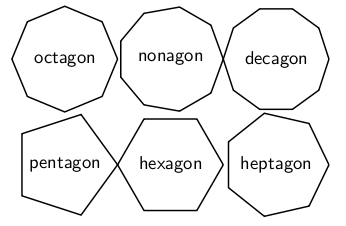
\includegraphics{col11306.imgs/m39368_MG10C13_046.png} % m39368;MG10C13\_046.png;;;6.0;8.5;
      \vspace{2pt}
    \vspace{\rubberspace}\par \begin{cnxcaption}
	  \small \textbf{Figure 12.47: }Examples of other polygons.
	\end{cnxcaption}
    \vspace{.1in}
    \rule[.1in]{\figurerulewidth}{.005in} \\
    \end{center}
 \end{figure}       
      \label{m39368*eip-210}
            \subsubsection{ Angles of Regular Polygons}
            \nopagebreak
            \label{m39368*id319627}Polygons need not have all sides the same. When they do, they are called regular polygons. You can calculate the size of the interior angle of a regular polygon by using:\par 
          \label{m39368*uid96}\nopagebreak\noindent{}
            
    \begin{equation}
    \hat{A}=\frac{n-2}{n}\ensuremath{\times}{180}^{\circ }\tag{12.5}
      \end{equation}
          \label{m39368*id319678}where $n$ is the number of sides and $\hat{A}$ is any angle.\par \label{m39368*eip-804}\vspace{.5cm} 
      \noindent
      \hspace*{-30pt}
\includegraphics[width=0.5in]{col11306.imgs/pspencil2.png}   \raisebox{25mm}{   
      \begin{mdframed}[linewidth=4, leftmargin=40, rightmargin=40]  
      \begin{exercise}
    \noindent\textbf{Exercise 12.4}\label{m39368*eip-708}
  \label{m39368*eip-618}
    Find the size of the interior angles of a regular octagon.
  \par 
\vspace{5pt}
\label{m39368*eip-937}\noindent\textbf{Solution to Exercise }
\label{m39368*id7432}\begin{enumerate}[noitemsep, label=\textbf{Step} \textbf{\arabic*}. ] 
            \leftskip=20pt\rightskip=\leftskip\item 
An octagon has 8 sides.
\item 
\label{m39368*id7344}\nopagebreak\noindent{}

    \begin{equation}
    \begin{array}{ccc}\hfill \hat{A}& =& \frac{n-2}{n}\ensuremath{\times}{180}^{\circ }\hfill \\ \hfill \hat{A}& =& \frac{8-2}{8}\ensuremath{\times}{180}^{\circ }\hfill \\ \hfill \hat{A}& =& \frac{6}{2}\ensuremath{\times}{180}^{\circ }\hfill \\ \hfill \hat{A}& =& {135}^{\circ }\hfill \end{array}\tag{12.6}
      \end{equation}
\end{enumerate}
    \end{exercise}
    \end{mdframed}
    }
    \noindent
%  **************GEOMETRY****************8  
%        
%          \section{ Polygons and quadrilaterals}
%     \nopagebreak
%             \label{m39354} $ \hspace{-5pt}\begin{array}{cccccccccccc}   
\includegraphics[width=0.75cm]{col11306.imgs/summary_fullmarks.png} &   \end{array} $ \hspace{2 pt}\raisebox{-5 pt}{} {(section shortcode: MG10093 )} \par 
%     
%     
    \label{m39354*cid2}
            \subsection{ Introduction}
            \nopagebreak
      \label{m39354*id62184}Geometry (Greek: geo = earth, metria = measure) arose as the field of knowledge dealing with spatial relationships. It was one of the two fields of pre-modern mathematics, the other being the study of numbers. In modern times, geometric concepts have become very complex and abstract and are barely recognizable as the descendants of early geometry. Geometry is often split into Euclidean geometry and analytical geometry. Euclidean geometry is covered in this chapter.\par 
% \label{m39354*secfhsst!!!underscore!!!id69}
%             \subsubsection{  Research Project : History of Geometry }
%             \nopagebreak
%             
%       \label{m39354*id62198}Work in pairs or groups and investigate the history of the foundation of geometry. Describe the various stages of development and how the following cultures used geometry to improve their lives. This list should serve as a guideline and provide the minimum requirement, there are many other people who contributed to the foundation of geometry.\par 
%       \label{m39354*id62543}\begin{enumerate}[noitemsep, label=\textbf{\arabic*}. ] 
%             \label{m39354*uid1}\item Ancient Indian geometry (c. 3000 - 500 B.C.)
% \label{m39354*id62557}\begin{enumerate}[noitemsep, label=\textbf{\alph*}. ] 
%             \label{m39354*uid2}\item Harappan geometry
% \label{m39354*uid3}\item Vedic geometry
% \end{enumerate}
%         \label{m39354*uid4}\item Classical Greek geometry (c. 600 - 300 B.C.)
% \label{m39354*id62596}\begin{enumerate}[noitemsep, label=\textbf{\alph*}. ] 
%             \label{m39354*uid5}\item Thales and Pythagoras
% \label{m39354*uid677}\item Plato
% \end{enumerate}
%         \label{m39354*uid787}\item Hellenistic geometry (c. 300 B.C - 500 C.E.)
% \label{m39354*id62634}\begin{enumerate}[noitemsep, label=\textbf{\alph*}. ] 
%             \label{m39354*uid887}\item Euclid
% \label{m39354*uid987}\item Archimedes
% \end{enumerate}
%         \end{enumerate}
%         
%       
    \label{m39354*uid52}
            \subsection{ Quadrilaterals}
            \nopagebreak
        \label{m39354*id974}In this section we will look at the properties of some special quadrilaterals. We will then use these properties to solve geometrical problems. It should be noted that although all the properties of a figure are given, we only need one unique property of the quadrilateral to prove that it is that quadrilateral. For example, if we have a quadrilateral with two pairs of opposite sides parallel, then that quadrilateral is a parallelogram. We can then prove the other properties of the quadrilateral using what we have learnt about parallel lines and triangles.\par 
        \label{m39354*uid54}
            \subsubsection{ Trapezium}
            \nopagebreak
          \label{m39354*id318803}A trapezium is a quadrilateral with one pair of parallel opposite sides. It may also be called a \textsl{trapezoid}. A special type of trapezium is the \textsl{isosceles trapezium}, where one pair of opposite sides is parallel, the other pair of sides is equal in length and the angles at the ends of each parallel side are equal. An isosceles trapezium has one line of symmetry and its diagonals are equal in length.\par 
          \label{m39354*eip-994}Note: The term trapezoid is predominantly used in North America and refers to what we call a trapezium. Rather confusingly, they use the term 'trapezium' to refer to a general irregular quadrilateral, that is a quadrilateral with no parallel sides!\par 
    \setcounter{subfigure}{0}
	\begin{figure}[H] % horizontal\label{m39354*uid55}
    \begin{center}
    \rule[.1in]{\figurerulewidth}{.005in} \\
        \label{m39354*uid55!!!underscore!!!media}\label{m39354*uid55!!!underscore!!!printimage}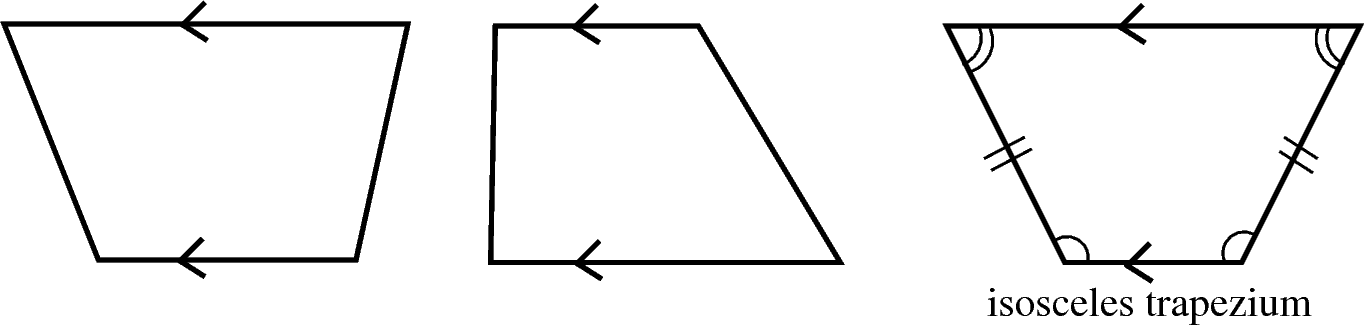
\includegraphics{col11306.imgs/m39354_MG10C13_040.png} % m39354;MG10C13\_040.png;;;6.0;8.5;
      \vspace{2pt}
    \vspace{\rubberspace}\par \begin{cnxcaption}
	  \small \textbf{Figure 13.1: }Examples of trapeziums.
	\end{cnxcaption}
    \vspace{.1in}
    \rule[.1in]{\figurerulewidth}{.005in} \\
    \end{center}
 \end{figure}       
        \label{m39354*uid56}
            \subsubsection{ Parallelogram}
            \nopagebreak
          \label{m39354*id318843}A trapezium with both sets of opposite sides parallel is called a \textsl{parallelogram}. A summary of the properties of a parallelogram is:\par 
          \label{m39354*id318853}\begin{itemize}[noitemsep]
            \label{m39354*uid57}\item Both pairs of opposite sides are parallel.
\label{m39354*uid58}\item Both pairs of opposite sides are equal in length.
\label{m39354*uid59}\item Both pairs of opposite angles are equal.
\label{m39354*uid60}\item Both diagonals bisect each other (i.e. they cut each other in half).
\end{itemize}
    \setcounter{subfigure}{0}
	\begin{figure}[H] % horizontal\label{m39354*uid61}
    \begin{center}
    \rule[.1in]{\figurerulewidth}{.005in} \\
        \label{m39354*uid61!!!underscore!!!media}\label{m39354*uid61!!!underscore!!!printimage}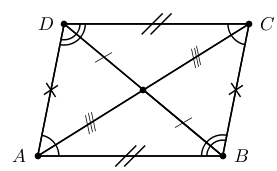
\includegraphics{col11306.imgs/m39354_MG10C13_041.png} % m39354;MG10C13\_041.png;;;6.0;8.5;
      \vspace{2pt}
    \vspace{\rubberspace}\par \begin{cnxcaption}
	  \small \textbf{Figure 13.2: }An example of a parallelogram.
	\end{cnxcaption}
    \vspace{.1in}
    \rule[.1in]{\figurerulewidth}{.005in} \\
    \end{center}
 \end{figure}       
        \label{m39354*uid62}
            \subsubsection{ Rectangle}
            \nopagebreak
          \label{m39354*id318929}A \textsl{rectangle} is a parallelogram that has all four angles equal to ${90}^{\circ }$. A summary of the properties of a rectangle is:\par 
          \label{m39354*id318954}\begin{itemize}[noitemsep]
            \label{m39354*uid63}\item Both pairs of opposite sides are parallel.
\label{m39354*uid64}\item Both pairs of opposite sides are of equal length.
\label{m39354*uid65}\item Both diagonals bisect each other.
\label{m39354*uid66}\item Diagonals are equal in length.
\label{m39354*uid67}\item All angles at the corners are right angles.
\end{itemize}
    \setcounter{subfigure}{0}
	\begin{figure}[H] % horizontal\label{m39354*uid68}
    \begin{center}
    \rule[.1in]{\figurerulewidth}{.005in} \\
        \label{m39354*uid68!!!underscore!!!media}\label{m39354*uid68!!!underscore!!!printimage}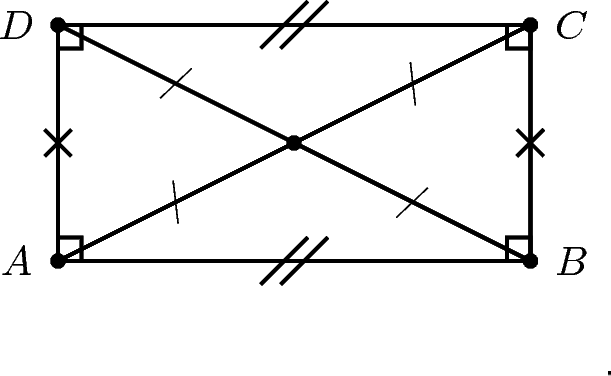
\includegraphics{col11306.imgs/m39354_MG10C13_042.png} % m39354;MG10C13\_042.png;;;6.0;8.5;
      \vspace{2pt}
    \vspace{\rubberspace}\par \begin{cnxcaption}
	  \small \textbf{Figure 13.3: }Example of a rectangle.
	\end{cnxcaption}
    \vspace{.1in}
    \rule[.1in]{\figurerulewidth}{.005in} \\
    \end{center}
 \end{figure}       
        \label{m39354*uid69}
            \subsubsection{ Rhombus}
            \nopagebreak
          \label{m39354*id319041}A \textsl{rhombus} is a parallelogram that has all four sides of equal length. A summary of the properties of a rhombus is:\par 
          \label{m39354*id319051}\begin{itemize}[noitemsep]
            \label{m39354*uid70}\item Both pairs of opposite sides are parallel.
\label{m39354*uid71}\item All sides are equal in length.
\label{m39354*uid72}\item Both pairs of opposite angles are equal.
\label{m39354*uid73}\item Both diagonals bisect each other at ${90}^{\circ }$.
\label{m39354*uid74}\item Diagonals of a rhombus bisect both pairs of opposite angles.
\end{itemize}
    \setcounter{subfigure}{0}
	\begin{figure}[H] % horizontal\label{m39354*uid75}
    \begin{center}
    \rule[.1in]{\figurerulewidth}{.005in} \\
        \label{m39354*uid75!!!underscore!!!media}\label{m39354*uid75!!!underscore!!!printimage}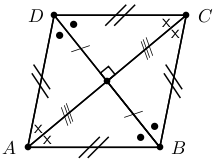
\includegraphics{col11306.imgs/m39354_MG10C13_043.png} % m39354;MG10C13\_043.png;;;6.0;8.5;
      \vspace{2pt}
    \vspace{\rubberspace}\par \begin{cnxcaption}
	  \small \textbf{Figure 13.4: }An example of a rhombus. A rhombus is a parallelogram with all sides equal.
	\end{cnxcaption}
    \vspace{.1in}
    \rule[.1in]{\figurerulewidth}{.005in} \\
    \end{center}
 \end{figure}       
        \label{m39354*uid76}
            \subsubsection{ Square}
            \nopagebreak
          \label{m39354*id319154}A \textsl{square} is a rhombus that has all four angles equal to 90${}^{\circ }$.\par 
          \label{m39354*id319177}A summary of the properties of a square is:\par 
          \label{m39354*id319181}\begin{itemize}[noitemsep]
            \label{m39354*uid77}\item Both pairs of opposite sides are parallel.
\label{m39354*uid78}\item All sides are equal in length.
\label{m39354*uid79}\item All angles are equal to ${90}^{\circ }$.
\label{m39354*uid80}\item Both pairs of opposite angles are equal.
\label{m39354*uid81}\item Both diagonals bisect each other at ${90}^{\circ }$.
\label{m39354*uid82}\item Diagonals are equal in length.
\label{m39354*uid83}\item Diagonals bisect both pairs of opposite angles (ie. all ${45}^{\circ }$).
\end{itemize}
    \setcounter{subfigure}{0}
	\begin{figure}[H] % horizontal\label{m39354*uid84}
    \begin{center}
    \rule[.1in]{\figurerulewidth}{.005in} \\
        \label{m39354*uid84!!!underscore!!!media}\label{m39354*uid84!!!underscore!!!printright prismsimage}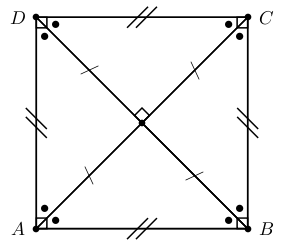
\includegraphics{col11306.imgs/m39354_MG10C13_044.png} % m39354;MG10C13\_044.png;;;6.0;8.5;
      \vspace{2pt}
    \vspace{\rubberspace}\par \begin{cnxcaption}
	  \small \textbf{Figure 13.5: }An example of a square. A square is a rhombus with all angles equal to 90${}^{\circ }$.
	\end{cnxcaption}
    \vspace{.1in}
    \rule[.1in]{\figurerulewidth}{.005in} \\
    \end{center}
 \end{figure}       
        \label{m39354*uid85}
            \subsubsection{ Kite}
            \nopagebreak
          \label{m39354*id319349}A \textsl{kite} is a quadrilateral with two pairs of adjacent sides equal.\par 
          \label{m39354*id319359}A summary of the properties of a kite is:\par 
          \label{m39354*id319362}\begin{itemize}[noitemsep]
            \label{m39354*uid86}\item Two pairs of adjacent sides are equal in length.
\label{m39354*uid87}\item One pair of opposite angles are equal where the angles are between unequal sides.
\label{m39354*uid88}\item One diagonal bisects the other diagonal and one diagonal bisects one pair of opposite angles.
\label{m39354*uid89}\item Diagonals intersect at right-angles.
\end{itemize}
    \setcounter{subfigure}{0}
	\begin{figure}[H] % horizontal\label{m39354*uid90}
    \begin{center}
    \rule[.1in]{\figurerulewidth}{.005in} \\
        \label{m39354*uid90!!!underscore!!!media}\label{m39354*uid90!!!underscore!!!printimage}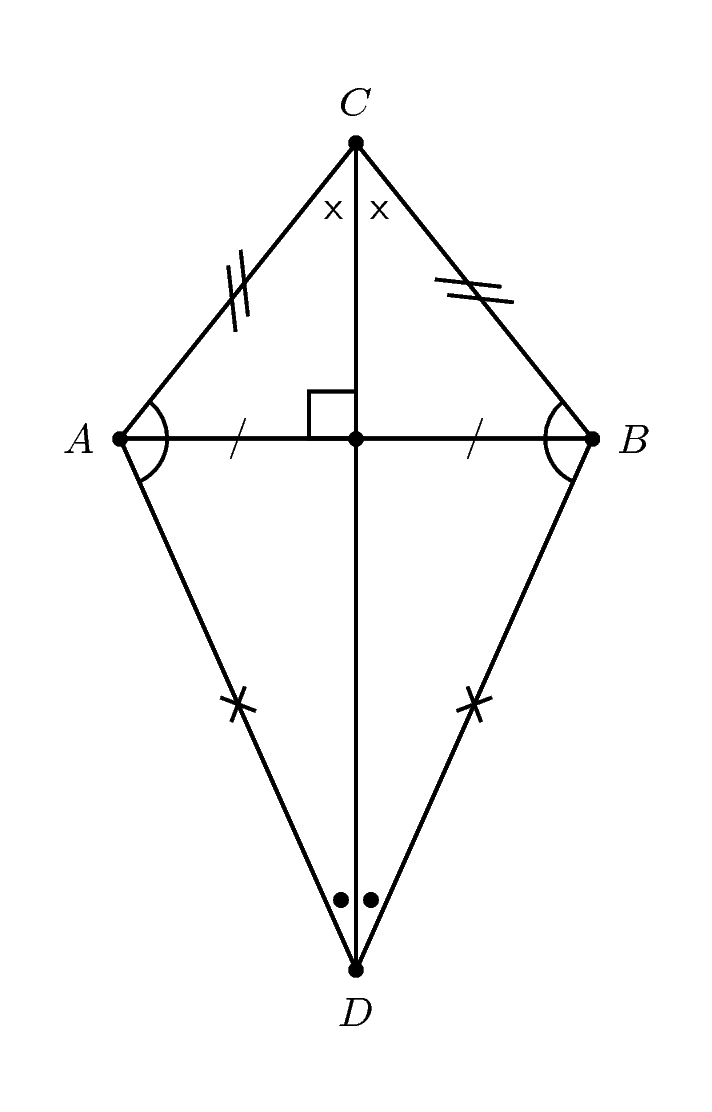
\includegraphics{col11306.imgs/m39354_MG10C13_045.png} % m39354;MG10C13\_045.png;;;6.0;8.5;
      \vspace{2pt}
    \vspace{\rubberspace}\par \begin{cnxcaption}
	  \small \textbf{Figure 13.6: }An example of a kite.
	\end{cnxcaption}
    \vspace{.1in}
    \rule[.1in]{\figurerulewidth}{.005in} \\
    \end{center}
 \end{figure}       
\label{m39354*id9732}Rectangles are a special case (or a subset) of parallelograms. Rectangles are parallelograms that have all angles equal to 90. Squares are a special case (or subset) of rectangles. Squares are rectangles that have all sides equal in length. So all squares are parallelograms and rectangles. So if you are asked to prove that a quadrilateral is a parallelogram, it is enough to show that both pairs of opposite sides are parallel. But if you are asked to prove that a quadrilateral is a square, then you must also show that the angles are all right angles and the sides are equal in length.
\par 
%       
%       \label{m39354*cid4}
%             \subsection{ Polygons}
%             \nopagebreak
%             
%       
%       \label{m39354*id64553}Polygons are all around us. A stop sign is in the shape of an octagon, an eight-sided polygon. The honeycomb of a beehive consists of hexagonal cells. The top of a desk is a rectangle. Note that although in the first two of these cases the sides of the polygon are all the same, but this need not be the case. Polygons with all sides and angles the same are called 'regular', while those with some sides or angles that are different are called 'irregular'. Although we often work with irregular triangles and quadrilaterals, once one gets up to polygons with greater than four sides, the more interesting ones are often the regular ones.\par 
%       \label{m39354*id64557}In this section, you will learn about similar polygons.\par 
%       \label{m39354*uid25}
%             \subsubsection{ Similarity of Polygons}
%             \nopagebreak
%             
%         
% \label{m39354*secfhsst!!!underscore!!!id491}
%             \subsubsection{  Discussion : Similar Triangles }
%             \nopagebreak
%             
%         \label{m39354*id64577}Fill in the table using the diagram and then answer the questions that follow.\par 
%         
%     % \textbf{m39354*id64584}\par
%     
%           \begin{table}
%         
%     % \begin{table}[H]
%     % \\ '' '0'
%     
%         \begin{center}
%       
%       \label{m39354*id64584}
%       
%     \noindent
%     \tabletail{%
%         \hline
%         \multicolumn{3}{|p{\mytableboxwidth}|}{\raggedleft \small \sl continued on next page}\\
%         \hline
%       }
%       \tablelasttail{}
%       \begin{xtabular}[t]{|l|l|l|}\hline
%     
%     
%         $\frac{\mathrm{AB}}{\mathrm{DE}}$=$\frac{...cm}{...cm}=...$ &
%     
%     
%         $\hat{A}$=...${}^{\circ }$ &
%     
%     
%         $\hat{D}$...${}^{\circ }$% make-rowspan-placeholders
%      \tabularnewline\cline{1-1}\cline{2-2}\cline{3-3}
%       %--------------------------------------------------------------------
%     
%     
%         $\frac{\mathrm{BC}}{\mathrm{EF}}$=$\frac{...cm}{...cm}=...$ &
%     
%     
%         $\hat{B}$=...${}^{\circ }$ &
%     
%     
%         $\hat{E}$=...${}^{\circ }$% make-rowspan-placeholders
%      \tabularnewline\cline{1-1}\cline{2-2}\cline{3-3}
%       %--------------------------------------------------------------------
%     
%     
%         $\frac{\mathrm{AC}}{\mathrm{DF}}$=$\frac{...cm}{...cm}=...$ &
%     
%     
%         $\hat{C}$...${}^{\circ }$ &
%     
%     
%         $\hat{F}$=...${}^{\circ }$% make-rowspan-placeholders
%      \tabularnewline\cline{1-1}\cline{2-2}\cline{3-3}
%       %--------------------------------------------------------------------
%     \end{xtabular}
%       \end{center}
%     \begin{center}{\small\bfseries Table 13.1}\end{center}
%     \begin{caption}{\small\bfseries Table 13.1}\end{caption}
\end{table}
%       
%     \par
%   
%         
%         \label{m39354*id65008}
%           
%     \setcounter{subfigure}{0}
% 
% 
% 	\begin{figure}[H] % horizontal\label{m39354*id65011}
%     \begin{center}
%     \label{m39354*id65011!!!underscore!!!media}\label{m39354*id65011!!!underscore!!!printimage}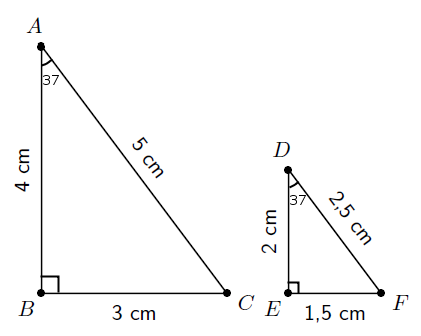
\includegraphics[width=300px]{col11306.imgs/m39354_MG10C14_010.png} % m39354;MG10C14\_010.png;;;6.0;8.5;
%         
%       \vspace{2pt}
%     \vspace{.1in}
%     
%     \end{center}
% 
%  \end{figure}   
% %     
%         \par 
%         \label{m39354*id65017}\begin{enumerate}[noitemsep, label=\textbf{\arabic*}. ] 
%             \label{m39354*uid26}\item What can you say about the numbers you calculated for: $\frac{\mathrm{AB}}{\mathrm{DE}}$, $\frac{\mathrm{BC}}{\mathrm{EF}}$, $\frac{\mathrm{AC}}{\mathrm{DF}}$?
% \label{m39354*uid27}\item What can you say about $\hat{A}$ and $\hat{D}$?
% \label{m39354*uid28}\item What can you say about $\hat{B}$ and $\hat{E}$?
% \label{m39354*uid29}\item What can you say about $\hat{C}$ and $\hat{F}$?
% \end{enumerate}
%         
%         
% 
%         \label{m39354*id65212}If two polygons are \textsl{similar}, one is an enlargement of the other. This means that the two polygons will have the same angles and their sides will be in the same proportion.\par 
%         \label{m39354*id65223}We use the symbol $|||$ to mean \textsl{is similar to}.\par 
% \label{m39354*fhsst!!!underscore!!!id537}\begin{definition}
% 	  \begin{tabular*}{15 cm}{m{15 mm}m{}}
% 	\hspace*{-50pt}  
\includegraphics[width=0.5in]{col11306.imgs/psflag2.png}   & \Definition{   \label{id2573375}\textbf{ Similar Polygons }} { \label{m39354*meaningfhsst!!!underscore!!!id537}
%         \label{m39354*id65247}Two polygons are similar if:\par 
%         \label{m39354*id65253}\begin{enumerate}[noitemsep, label=\textbf{\arabic*}. ] 
%             \leftskip=20pt\rightskip=\leftskip\label{m39354*uid30}\item their corresponding angles are equal, \textbf{and}\label{m39354*uid31}\item the ratios of corresponding sides are equal.
% \end{enumerate}
%         
%         
%          } 
%       \end{tabular*}
%       \end{definition}
% 
% \par
%             \label{m39354*secfhsst!!!underscore!!!id546}\vspace{.5cm} 
%       
%       \noindent
%       \hspace*{-30pt}
\includegraphics[width=0.5in]{col11306.imgs/pspencil2.png}   \raisebox{25mm}{   
%       \begin{mdframed}[linewidth=4, leftmargin=40, rightmargin=40]  
%       \begin{exercise}
%     \noindent\textbf{Exercise 13.1:  Similarity of Polygons }
%         \label{m39354*probfhsst!!!underscore!!!id547}
%         \label{m39354*id65309}Show that the following two polygons are similar.\par 
%         \label{m39354*id65315}
%           
%     \setcounter{subfigure}{0}
% 
% 
% 	\begin{figure}[H] % horizontal\label{m39354*id65318}
%     \begin{center}
%     \label{m39354*id65318!!!underscore!!!media}\label{m39354*id65318!!!underscore!!!printimage}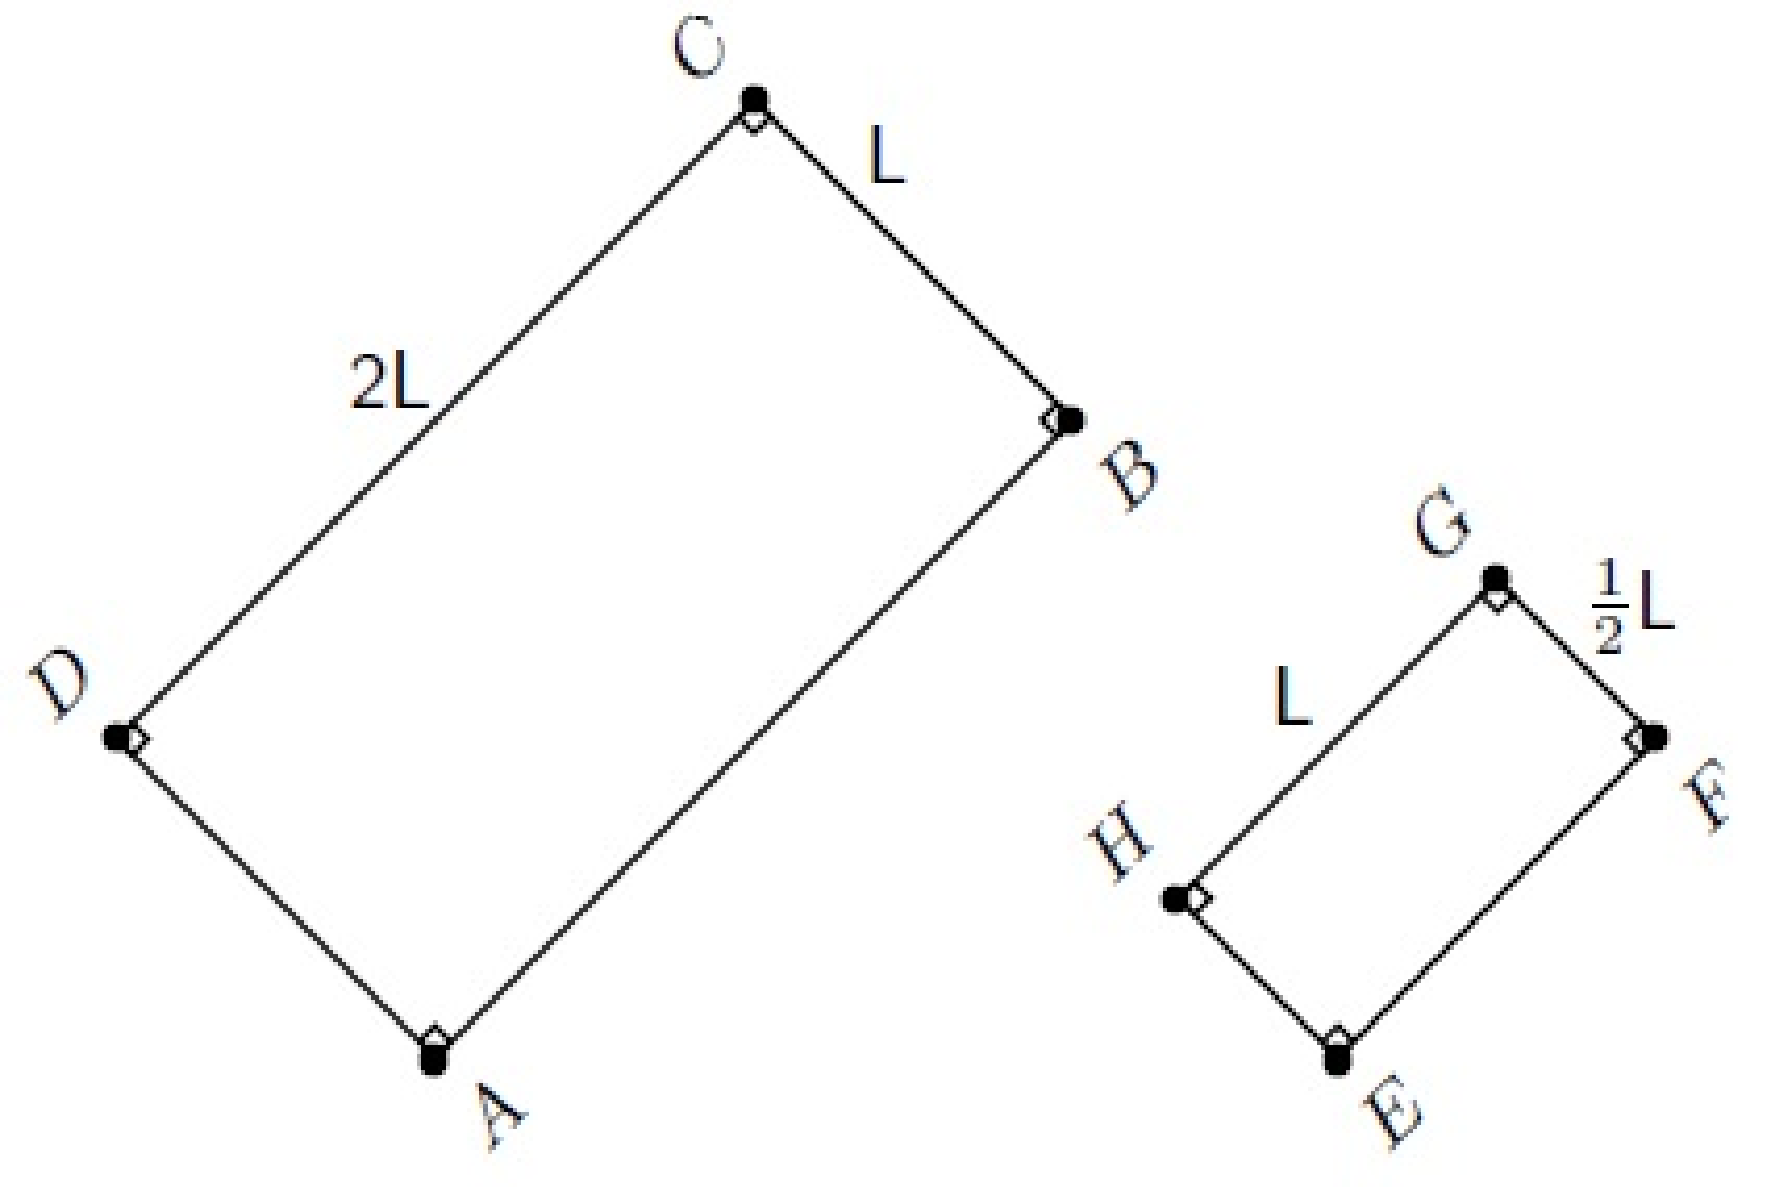
\includegraphics[width=300px]{col11306.imgs/m39354_MG10C14_011.png} % m39354;MG10C14\_011.png;;;6.0;8.5;
%         
%       \vspace{2pt}
%     \vspace{.1in}
%     
%     \end{center}
% 
%  \end{figure}   
% %     
%         \par 
%         
%         \vspace{5pt}
%         \label{m39354*solfhsst!!!underscore!!!id559}\noindent\textbf{Solution to Exercise } \label{m39354*listfhsst!!!underscore!!!id559}\begin{enumerate}[noitemsep, label=\textbf{Step} \textbf{\arabic*}. ] 
%             \leftskip=20pt\rightskip=\leftskip\item  
%         \label{m39354*id65346}We are required to show that the pair of polygons is similar. We can do this by showing that the ratio of corresponding sides is equal and by showing that corresponding angles are equal.\par 
%         \item  
%         \label{m39354*id65355}We are given the angles. So, we can show that corresponding angles are equal.\par 
%         \item  
%         \label{m39354*id65363}All angles are given to be 90${}^{\circ }$ and\par 
%         \label{m39354*id65380}\nopagebreak\noindent{}
%           
%     \begin{equation}
%     \begin{array}{ccc}\hfill \hat{A}& =& \hat{E}\hfill \\ \hfill \hat{B}& =& \hat{F}\hfill \\ \hfill \hat{C}& =& \hat{G}\hfill \\ \hfill \hat{D}& =& \hat{H}\hfill \end{array}\tag{13.1}
%       \end{equation}
%     
%         
%         \item  
%         \label{m39354*id65511}We first need to see which sides correspond. The rectangles have two equal long sides and two equal short sides. We need to compare the ratio of the long side lengths of the two different rectangles as well as the ratio of the short side lenghts.\par 
%         \label{m39354*id65517}Long sides, large rectangle values over small rectangle values:\par 
%         \label{m39354*id65521}\nopagebreak\noindent{}
%     \begin{equation}
%     \begin{array}{ccc}\hfill \mathrm{Ratio}& =& \frac{2L}{L}\hfill \\ & =& 2\hfill \end{array}\tag{13.2}
%       \end{equation}
%     
%         
%         \label{m39354*id65569}Short sides, large rectangle values over small rectangle values:\par 
%         \label{m39354*id65572}\nopagebreak\noindent{}
%     \begin{equation}
%     \begin{array}{ccc}\hfill \mathrm{Ratio}& =& \frac{L}{\frac{1}{2}L}\hfill \\ & =& \frac{1}{\frac{1}{2}}\hfill \\ & =& 2\hfill \end{array}\tag{13.3}
%       \end{equation}
%     
%         
%         \label{m39354*id65644}The ratios of the corresponding sides are equal, 2 in this case.\par 
%         \item  
%         \label{m39354*id65652}Since corresponding angles are equal and the ratios of the corresponding sides are equal the polygons ABCD and EFGH are similar. \par 
%         \end{enumerate}
%          
% 
%     \end{exercise}
%     \end{mdframed}
%     }
%     \noindent
%   
% \label{m39354*notfhsst!!!underscore!!!id731}
% \begin{tabular}{cc}
% 	   \hspace*{-50pt}\raisebox{-8 mm}{ 
\includegraphics[width=0.5in]{col11306.imgs/pstip2.png}  }& 
% 
% 	\begin{minipage}{0.85\textwidth}
% 	\begin{note}
%       {tip: }All squares are similar.
% 	\end{note}
% 	\end{minipage}
% 	\end{tabular}
% 	\par
%       
% \label{m39354*secfhsst!!!underscore!!!id732}\vspace{.5cm} 
%       
%       \noindent
%       \hspace*{-30pt}
\includegraphics[width=0.5in]{col11306.imgs/pspencil2.png}   \raisebox{25mm}{   
%       \begin{mdframed}[linewidth=4, leftmargin=40, rightmargin=40]  
%       \begin{exercise}
%     \noindent\textbf{Exercise 13.2:  Similarity of Polygons }
%         \label{m39354*probfhsst!!!underscore!!!id733}
%         \label{m39354*id65687}If two pentagons ABCDE and GHJKL are similar, determine the lengths of the sides and angles labelled with letters:\par 
%         \label{m39354*id65694}
%           
%     \setcounter{subfigure}{0}
% 
% 
% 	\begin{figure}[H] % horizontal\label{m39354*id65697}
%     \begin{center}
%     \label{m39354*id65697!!!underscore!!!media}\label{m39354*id65697!!!underscore!!!printimage}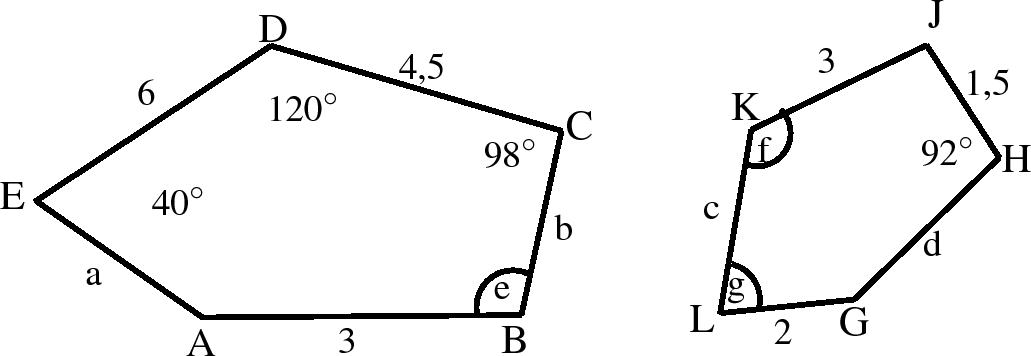
\includegraphics[width=300px]{col11306.imgs/m39354_MG10C14_012.png} % m39354;MG10C14\_012.png;;;6.0;8.5;
%         
%       \vspace{2pt}
%     \vspace{.1in}
%     
%     \end{center}
% 
%  \end{figure}   
% %     
%         \par 
%         
%         \vspace{5pt}
%         \label{m39354*solfhsst!!!underscore!!!id745}\noindent\textbf{Solution to Exercise } \label{m39354*listfhsst!!!underscore!!!id745}\begin{enumerate}[noitemsep, label=\textbf{Step} \textbf{\arabic*}. ] 
%             \leftskip=20pt\rightskip=\leftskip\item  
%         \label{m39354*id65725}We are given that ABCDE and GHJKL are similar. This means that:\par 
%         \label{m39354*id65729}\nopagebreak\noindent{}
%           
%     \begin{equation}
%     \frac{\mathrm{AB}}{\mathrm{GH}}=\frac{\mathrm{BC}}{\mathrm{HJ}}=\frac{\mathrm{CD}}{\mathrm{JK}}=\frac{\mathrm{DE}}{\mathrm{KL}}=\frac{\mathrm{EA}}{\mathrm{LG}}\tag{13.4}
%       \end{equation}
%     
%         
%         \label{m39354*id65782}and\par 
%         \label{m39354*id65787}\nopagebreak\noindent{}
%           
%     \begin{equation}
%     \begin{array}{ccc}\hfill \hat{A}& =& \hat{G}\hfill \\ \hfill \hat{B}& =& \hat{H}\hfill \\ \hfill \hat{C}& =& \hat{J}\hfill \\ \hfill \hat{D}& =& \hat{K}\hfill \\ \hfill \hat{E}& =& \hat{L}\hfill \end{array}\tag{13.5}
%       \end{equation}
%     
%         
%         \item  
%         \label{m39354*id65948}We are required to determine the\par 
%         \label{m39354*id65951}\begin{enumerate}[noitemsep, label=\textbf{\alph*}. ] 
%             \leftskip=20pt\rightskip=\leftskip\label{m39354*uid32}\item $a$, $b$, $c$ and $d$, and
% \label{m39354*uid33}\item $e$, $f$ and $g$.
% \end{enumerate}
%         
%         \item  
%         \label{m39354*id66048}The corresponding angles are equal, so no calculation is needed. We are given one pair of sides $DC$ and $KJ$ that correspond. $\frac{DC}{KJ}=\frac{4,5}{3}=1,5$ so we know that all sides of $KJHGL$ are 1,5 times smaller than $ABCDE$.\par 
%         \item  
%         \label{m39354*id66160}\nopagebreak\noindent{}
%           
%     \begin{equation}
%     \begin{array}{ccc}\hfill \frac{a}{2}=1,5& \therefore & a=2\ensuremath{\times}1,5=3\hfill \\ \hfill \frac{b}{1,5}=1,5& \therefore & b=1,5\ensuremath{\times}1,5=2,25\hfill \\ \hfill \frac{6}{c}=1,5& \therefore & c=6÷1,5=4\hfill \\ \hfill d=\frac{3}{1,5}& \therefore & d=2\hfill \end{array}\tag{13.6}
%       \end{equation}
%     
%         
%         \item  
%         \label{m39354*id66368}\nopagebreak\noindent{}
%     \begin{equation}
%     \begin{array}{ccc}\hfill e& =& {92}^{\circ }\left(\mathrm{corresponds\; to\; H}\right)\hfill \\ \hfill f& =& {120}^{\circ }\left(\mathrm{corresponds\; to\; D}\right)\hfill \\ \hfill g& =& {40}^{\circ }\left(\mathrm{corresponds\; to\; E}\right)\hfill \end{array}\tag{13.7}
%       \end{equation}
%     
%         
%         \item  
%         \label{m39354*id66506}\nopagebreak\noindent{}
%           
%     \begin{equation}
%     \begin{array}{ccc}\hfill a& =& 3\hfill \\ \hfill b& =& 2,25\hfill \\ \hfill c& =& 4\hfill \\ \hfill d& =& 2\hfill \\ \hfill e& =& {92}^{\circ }\hfill \\ \hfill f& =& {120}^{\circ }\hfill \\ \hfill g& =& {40}^{\circ }\hfill \end{array}\tag{13.8}
%       \end{equation}
%     
%         
%         
%         \end{enumerate}
%          
% 
%     \end{exercise}
%     \end{mdframed}
%     }
%     \noindent
%   
% \label{m39354*secfhsst!!!underscore!!!id1187}
%             \subsubsection{ Activity: Similarity of Equilateral Triangles }
%             \nopagebreak
%             
% \label{m39354*uid34283409} Working in pairs, show that all equilateral triangles are similar. \par 
%         
% 
% \label{m39354*secfhsst!!!underscore!!!id1190}
%             \subsubsection{  Polygons-mixed }
%             \nopagebreak
%             
%         \label{m39354*id66690}\begin{enumerate}[noitemsep, label=\textbf{\arabic*}. ] 
%             \label{m39354*uid34}\item Find the values of the unknowns in each case. Give reasons.
% 
%     \setcounter{subfigure}{0}
% 
% 
% 	\begin{figure}[H] % horizontal\label{m39354*id66710}
%     \begin{center}
%     \label{m39354*id66710!!!underscore!!!media}\label{m39354*id66710!!!underscore!!!printimage}\includegraphics{col11306.imgs/m39354_mg10c14_2.png} % m39354;mg10c14\_2.png;;;6.0;8.5;
%         
%       \vspace{2pt}
%     \vspace{.1in}
%     
%     \end{center}
% 
%  \end{figure}   
% %             \label{m39354*uid35}\item 
% Find the angles and lengths marked with letters in the following figures:
% 
%     \setcounter{subfigure}{0}
% 
% 
% 	\begin{figure}[H] % horizontal\label{m39354*id66733}
%     \begin{center}
%     \label{m39354*id66733!!!underscore!!!media}\label{m39354*id66733!!!underscore!!!printimage}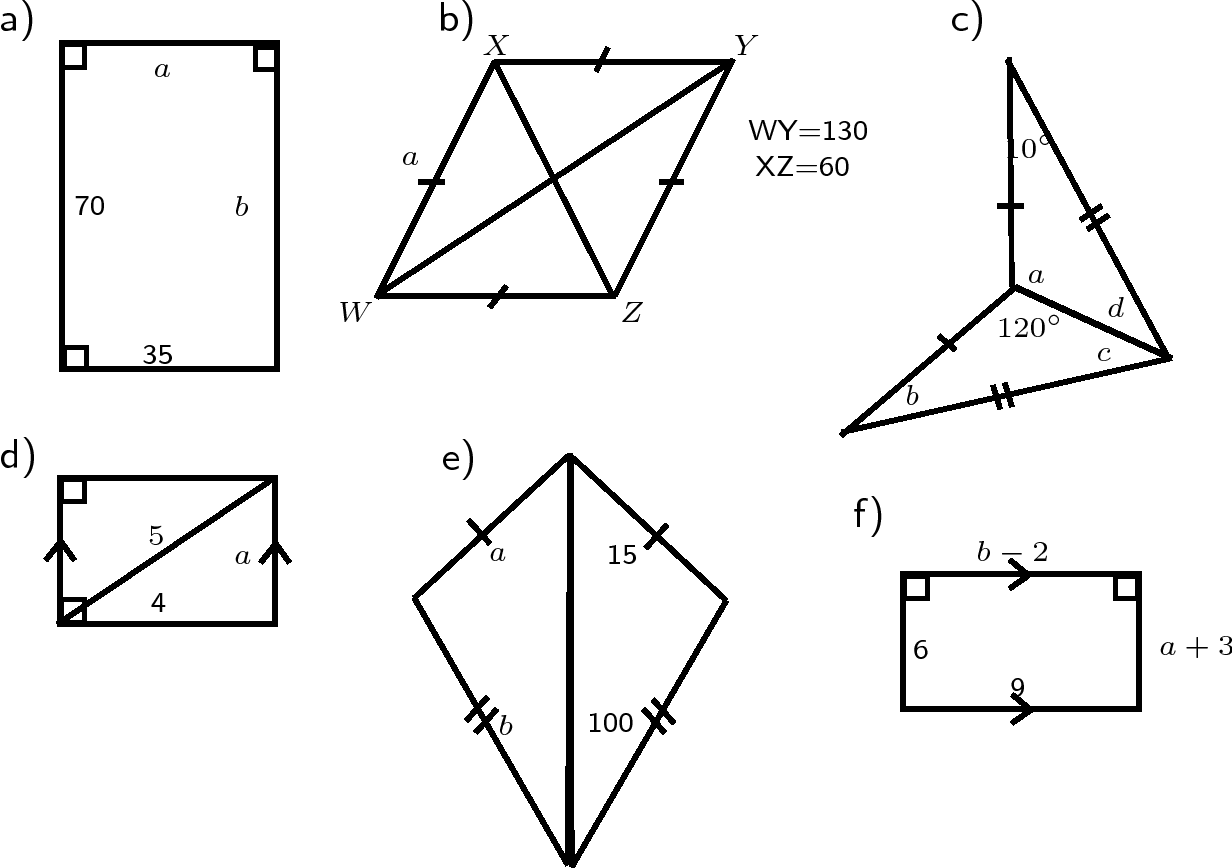
\includegraphics[width=300px]{col11306.imgs/m39354_MG10C14_014.png} % m39354;MG10C14\_014.png;;;6.0;8.5;
%         
%       \vspace{2pt}
%     \vspace{.1in}
%     
%     \end{center}
% 
%  \end{figure}   
% %             \end{enumerate}
%         
%         
% 
%       
%     
%       \label{m39354*eip-824}
% \par \raisebox{-5 pt}{
\includegraphics[width=0.5cm]{col11306.imgs/summary_www.png}} Find the answers with the shortcodes:
%  \par \begin{tabular}[h]{cccccc}
%  (1.) liD  &  (2.) liW  & \end{tabular}
% 
% 
% 
%             \subsection{ Investigation: Defining polygons}
%             \nopagebreak
%             \label{m39354*eip-779}Investigate the different ways of defining polygons. Polygons that you should pay special attention to are: \label{m39354*id6342}\begin{itemize}[noitemsep]
%             \item Isoceles, equilateral and right-angled triangle\item Kites, parallelograms, rectangles, rhombuses (or 'rhombi'), squares and trapeziums\end{itemize}
%         
% \par 
% \label{m39354*id7342}
% Things to consider are how these figures have been defined in this book and what alternative definitions exist. For example, a triangle is a three-sided polygon or a figure having three sides and three angles. Triangles can be classified using either their sides or their angles. Could you also classify quadrilaterals in this way? What other names exist for these figures? For example, quadrilaterals can also be called tetragons.
% \par 
% 
%   \label{m39354**end}
%          \section{ Proofs and conjectures}
%     \nopagebreak
%             \label{m39352} $ \hspace{-5pt}\begin{array}{cccccccccccc}   
\includegraphics[width=0.75cm]{col11306.imgs/summary_fullmarks.png} &   \end{array} $ \hspace{2 pt}\raisebox{-5 pt}{} {(section shortcode: MG10094 )} \par 
%     
%     
%     
\label{m39352*secfhsst!!!underscore!!!id933}
            \subsection{ Proofs and conjectures in geometry}
            \nopagebreak
            \label{m39352*id0723}You have seen how to use geometry and the properties of polygons to help you find unknown lengths and angles in various quadrilaterals and polygons. We will now extend this work to proving some of the properties and to solving riders. A conjecture is the mathematicians way of saying I believe that this is true, but I have no proof. The following worked examples will help make this clearer. 
\par 
\label{m39352*probfhsst!!!underscore!!!id072}\vspace{.5cm} 
      \noindent
      \hspace*{-30pt}
\includegraphics[width=0.5in]{col11306.imgs/pspencil2.png}   \raisebox{25mm}{   
      \begin{mdframed}[linewidth=4, leftmargin=40, rightmargin=40]  
      \begin{exercise}
    \noindent\textbf{Exercise 13.3: Proofs - 1}\label{m39352*id97832}\label{m39352*id943}Given quadrilateral ABCD, with $AB\parallel CD$ and $AD\parallel BC$, prove that $B\hat{A}D=B\hat{C}A$ and $A\hat{B}C=A\hat{D}C$.\par 
\vspace{5pt}
\label{m39352*solfhsst!!!underscore!!!id083}\noindent\textbf{Solution to Exercise }\label{m39352*id08324}\begin{enumerate}[noitemsep, label=\textbf{Step} \textbf{\arabic*}. ] 
            \leftskip=20pt\rightskip=\leftskip\item We draw the following diagram and construct the diagonals.
    \setcounter{subfigure}{0}
	\begin{figure}[H] % horizontal\label{m39352*uid310}
    \begin{center}
    \label{m39352*id897}\label{m39352*uid310!!!underscore!!!printimage}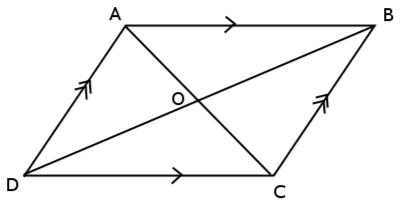
\includegraphics{col11306.imgs/m39352_geomproof1.png} % ;geomproof1.png;;;6.0;8.5;
      \vspace{2pt}
    \vspace{.1in}
    \end{center}
 \end{figure}       
\item Given: $AB\parallel CD$ and $AD\parallel BC$. We need to prove $A=C$ and $B=D$. In the formal language of maths we say that we are required to prove (RTP) $B\hat{A}D=B\hat{C}A$ and $A\hat{B}C=A\hat{D}C$. \item \label{m39352*id3468}\nopagebreak\noindent{}
    \begin{equation}
    \begin{array}{cccc}\hfill B\hat{A}C& =& A\hat{C}D\hfill & \left(\mathrm{corresponding\; angles}\right)\\ \hfill D\hat{A}C& =& B\hat{C}A\hfill & \left(\mathrm{corresponding\; angles}\right)\\ \hfill B\hat{A}D& =& B\hat{C}A\hfill & \end{array}\tag{13.9}
      \end{equation}
Similarly we find that: 
\label{m39352*id97}\nopagebreak\noindent{}
    \begin{equation}
    A\hat{B}C=A\hat{D}C\tag{13.10}
      \end{equation}
\end{enumerate}
    \end{exercise}
    \end{mdframed}
    }
    \noindent
\par
            \label{m39352*probfhsst!!!underscore!!!id073}\vspace{.5cm} 
      \noindent
      \hspace*{-30pt}
\includegraphics[width=0.5in]{col11306.imgs/pspencil2.png}   \raisebox{25mm}{   
      \begin{mdframed}[linewidth=4, leftmargin=40, rightmargin=40]  
      \begin{exercise}
    \noindent\textbf{Proofs - 2 13.4}
\label{m39352*id973452}\label{m39352*id95433}In parallelogram ABCD, the bisectors of the angles (AW, BX, CY and DZ) have been constructed:
    \setcounter{subfigure}{0}
	\begin{figure}[H] % horizontal\label{m39352*uid4140}
    \begin{center}
    \label{m39352*uid4140!!!underscore!!!media}\label{m39352*uid4140!!!underscore!!!printimage}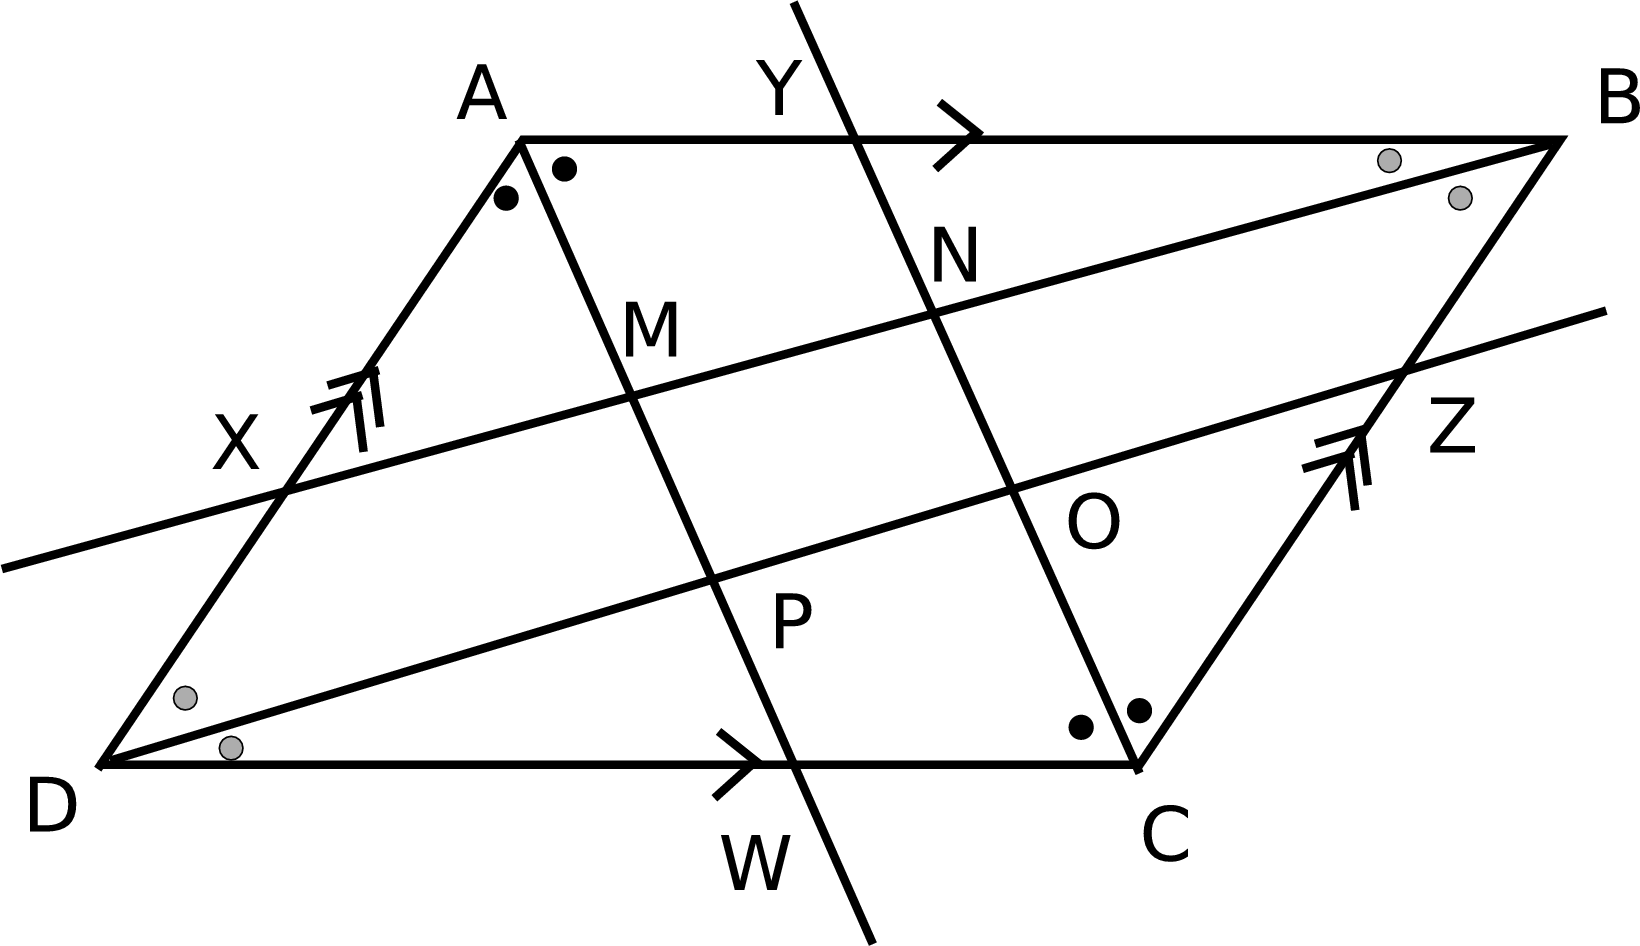
\includegraphics[width=300px]{col11306.imgs/m39352_geomproof2.png} % m39352;geomproof2.png;;;6.0;8.5;
      \vspace{2pt}
    \vspace{.1in}
    \end{center}
 \end{figure}       
You are also given that $\mathrm{AB}=\mathrm{CD}$, $\mathrm{AD}=\mathrm{BC}$, $\mathrm{AB}\parallel \mathrm{CD}$, $\mathrm{AD}\parallel \mathrm{BC}$,  $\hat{A}=\hat{C}$, and $\hat{B}=\hat{D}$. 
Prove that MNOP is a parallelogram.\par 
\vspace{5pt}
\label{m39352*solfhsst!!!underscore!!!id023}\noindent\textbf{Solution to Exercise }\label{m39352*id085424}\begin{enumerate}[noitemsep, label=\textbf{Step} \textbf{\arabic*}. ] 
            \leftskip=20pt\rightskip=\leftskip\item Given: $\mathrm{AB}=\mathrm{CD}$, $\mathrm{AD}=\mathrm{BC}$, $\mathrm{AB}\parallel \mathrm{CD}$, $\mathrm{AD}\parallel \mathrm{BC}$,  $\hat{A}=\hat{C}$, and $\hat{B}=\hat{D}$. RTP: MNOP is a parallelogram.\item 
\label{m39352*id368}\nopagebreak\noindent{}
    \begin{equation}
    \begin{array}{cc}\hfill In\phantom{\rule{2pt}{0ex}}▵\phantom{\rule{2pt}{0ex}}\mathrm{ADW}\phantom{\rule{2pt}{0ex}}\mathrm{and}\phantom{\rule{2pt}{0ex}}▵\mathrm{CBY}\phantom{\rule{2pt}{0ex}}\\ \hfill D\hat{A}W& =& B\hat{C}Y\phantom{\rule{2pt}{0ex}}\left(\mathrm{given}\right)\hfill \\ \hfill A\hat{D}C& =& A\hat{B}C\phantom{\rule{2pt}{0ex}}\left(\mathrm{given}\right)\hfill \\ \hfill \mathrm{AD}& =& \mathrm{BC}\phantom{\rule{2pt}{0ex}}\mathrm{\left(given\right)}\hfill \\ \hfill \therefore \phantom{\rule{2pt}{0ex}}▵\mathrm{ADW}& =& ▵\mathrm{CBY}\phantom{\rule{2pt}{0ex}}\mathrm{\left(AAS\right)}\hfill \\ \hfill \therefore \phantom{\rule{2pt}{0ex}}\mathrm{DW}& =& \mathrm{BY}\hfill \end{array}\tag{13.11}
      \end{equation}
\label{m39352*id378}\nopagebreak\noindent{}
    \begin{equation}
    \begin{array}{cc}\hfill In\phantom{\rule{2pt}{0ex}}▵\phantom{\rule{2pt}{0ex}}\mathrm{ABX}\phantom{\rule{2pt}{0ex}}\mathrm{and}\phantom{\rule{2pt}{0ex}}▵\mathrm{CDZ}\phantom{\rule{2pt}{0ex}}\\ \hfill D\hat{C}Z& =& B\hat{A}X\phantom{\rule{2pt}{0ex}}\left(\mathrm{given}\right)\hfill \\ \hfill Z\hat{D}C& =& X\hat{B}A\phantom{\rule{2pt}{0ex}}\left(\mathrm{given}\right)\hfill \\ \hfill \mathrm{DC}& =& \mathrm{AB}\phantom{\rule{2pt}{0ex}}\mathrm{\left(given\right)}\hfill \\ \hfill \therefore \phantom{\rule{2pt}{0ex}}▵\mathrm{ABX}& \equiv & ▵\mathrm{CDZ}\phantom{\rule{2pt}{0ex}}\mathrm{\left(AAS\right)}\hfill \\ \hfill \therefore \phantom{\rule{2pt}{0ex}}\mathrm{AX}& =& \mathrm{CZ}\hfill \end{array}\tag{13.12}
      \end{equation}
\label{m39352*id38868}\nopagebreak\noindent{}
    \begin{equation}
    \begin{array}{cc}\hfill In\phantom{\rule{2pt}{0ex}}▵\phantom{\rule{2pt}{0ex}}\mathrm{XAM}\phantom{\rule{2pt}{0ex}}\mathrm{and}\phantom{\rule{2pt}{0ex}}▵\mathrm{ZCO}\phantom{\rule{2pt}{0ex}}\\ \hfill X\hat{A}M& =& Z\hat{C}O\phantom{\rule{2pt}{0ex}}\left(\mathrm{given}\right)\hfill \\ \hfill A\hat{X}M& =& C\hat{Z}O\phantom{\rule{2pt}{0ex}}\left(\mathrm{proven\; above}\right)\hfill \\ \hfill \mathrm{AX}& =& \mathrm{CZ}\phantom{\rule{2pt}{0ex}}\mathrm{\left(proven\; above\right)}\hfill \\ \hfill \therefore \phantom{\rule{2pt}{0ex}}▵\mathrm{XAM}& \equiv & ▵\mathrm{COZ}\phantom{\rule{2pt}{0ex}}\mathrm{\left(AAS\right)}\hfill \\ \hfill \therefore \phantom{\rule{2pt}{0ex}}A\hat{O}C& =& A\hat{M}X\hfill \end{array}\tag{13.13}
      \end{equation}
\label{m39352*eip-914}\nopagebreak\noindent{}
    \begin{equation}
    \begin{array}{ccc}\hfill A\hat{M}X& =& P\hat{M}N\phantom{\rule{2pt}{0ex}}\mathrm{\left(vert.\; opp.\; \angle \text{'}s\right)}\hfill \\ \hfill C\hat{O}Z& =& N\hat{O}P\phantom{\rule{2pt}{0ex}}\mathrm{\left(vert.\; opp.\; \angle \text{'}s\right)}\hfill \\ \hfill \therefore \phantom{\rule{2pt}{0ex}}P\hat{M}N& =& N\hat{O}P\hfill \end{array}\tag{13.14}
      \end{equation}
    \label{m39352*id3838}\nopagebreak\noindent{}
    \begin{equation}
    \begin{array}{cc}\hfill In\phantom{\rule{2pt}{0ex}}▵\phantom{\rule{2pt}{0ex}}\mathrm{BYN}\phantom{\rule{2pt}{0ex}}\mathrm{and}\phantom{\rule{2pt}{0ex}}▵\mathrm{DWP}\phantom{\rule{2pt}{0ex}}\\ \hfill Y\hat{B}N& =& W\hat{D}P\phantom{\rule{2pt}{0ex}}\left(\mathrm{given}\right)\hfill \\ \hfill B\hat{Y}N& =& W\hat{D}P\phantom{\rule{2pt}{0ex}}\left(\mathrm{proven\; above}\right)\hfill \\ \hfill \mathrm{DW}& =& \mathrm{BY}\phantom{\rule{2pt}{0ex}}\mathrm{\left(proven\; above\right)}\hfill \\ \hfill \therefore \phantom{\rule{2pt}{0ex}}▵\mathrm{YBN}& \equiv & ▵\mathrm{WDP}\phantom{\rule{2pt}{0ex}}\mathrm{\left(AAS\right)}\hfill \\ \hfill \therefore \phantom{\rule{2pt}{0ex}}B\hat{N}Y& =& D\hat{P}W\hfill \end{array}\tag{13.15}
      \end{equation}
        \label{m39352*eip-557}\nopagebreak\noindent{}
    \begin{equation}
    \begin{array}{ccc}\hfill D\hat{P}W& =& M\hat{P}O\phantom{\rule{2pt}{0ex}}\mathrm{\left(vert.\; opp.\; \angle \text{'}s\right)}\hfill \\ \hfill B\hat{N}Y& =& O\hat{N}M\phantom{\rule{2pt}{0ex}}\mathrm{\left(vert.\; opp.\; \angle \text{'}s\right)}\hfill \\ \hfill \therefore \phantom{\rule{2pt}{0ex}}M\hat{P}O& =& O\hat{N}M\hfill \end{array}\tag{13.16}
      \end{equation}
    \label{m39352*eip-519}$\therefore $ MNOP is a parallelogram (both pairs opp. $\angle $'s $=$, and therefore both pairs opp. sides parallel too)\par 
\end{enumerate}
    \end{exercise}
    \end{mdframed}
    }
    \noindent
\label{m39352*id97342}
\begin{tabular}{cc}
	\hspace*{-50pt}\raisebox{-8 mm}{\hspace{-0.2in}
\includegraphics[width=0.75in]{col11306.imgs/psfact2.png} } & 
	\begin{minipage}{0.85\textwidth}
	\begin{note}
      {warning: }It is very important to note that a single counter example disproves a conjecture. Also numerous specific supporting examples do not prove a conjecture. 
	\end{note}
	\end{minipage}
	\end{tabular}
	\par
  \label{m39352**end}
%           
%          \section{ Measurement}
%     \nopagebreak
%             \label{m39357} $ \hspace{-5pt}\begin{array}{cccccccccccc}   
\includegraphics[width=0.75cm]{col11306.imgs/summary_fullmarks.png} &   
\includegraphics[width=0.75cm]{col11306.imgs/summary_video.png} &   \end{array} $ \hspace{2 pt}\raisebox{-5 pt}{} {(section shortcode: MG10095 )} \par 
%     
%     
%     
%     
%          \section{ Transformations}
%     \nopagebreak
%             \label{m39358} $ \hspace{-5pt}\begin{array}{cccccccccccc}   
\includegraphics[width=0.75cm]{col11306.imgs/summary_fullmarks.png} &   \end{array} $ \hspace{2 pt}\raisebox{-5 pt}{} {(section shortcode: MG10099 )} \par 
%     
%     
%     
%     
%    
%   \label{m39358*cid6}
%             \subsection{ Transformations - Enrichment, not in CAPS}
%             \nopagebreak
%             
%       
%       \label{m39358*id70076}In this section you will learn about how the co-ordinates of a point change when the point is moved horizontally and vertically on the Cartesian plane. You will also learn about what happens to the co-ordinates of a point when it is reflected on the $x$-axis, $y$-axis and the line $y=x$.\par 
%       \label{m39358*uid569}
%             \subsubsection{ Translation of a Point}
%             \nopagebreak
%             
%         
%         \label{m39358*id70123}When something is moved in a straight line, we say that it is \textsl{translated}. You will recall that the term 'translation' was also mentioned in the section on functions to refer to what happens when an entire function is shifted in a straight line. What happens to the co-ordinates of a point that is translated horizontally or vertically?\par 
% \label{m39358*secfhsst!!!underscore!!!id2414}
%             \subsubsection{  Discussion : Translation of a Point Vertically }
%             \nopagebreak
%             
%         \label{m39358*id70140}Complete the table, by filling in the co-ordinates of the points shown in the figure.\par 
%         \label{m39358*id70146}
%           
%     \setcounter{subfigure}{0}
% 
% 
% 	\begin{figure}[H] % horizontal\label{m39358*id70150}
%     \begin{center}
%     \label{m39358*id70150!!!underscore!!!media}\label{m39358*id70150!!!underscore!!!printimage}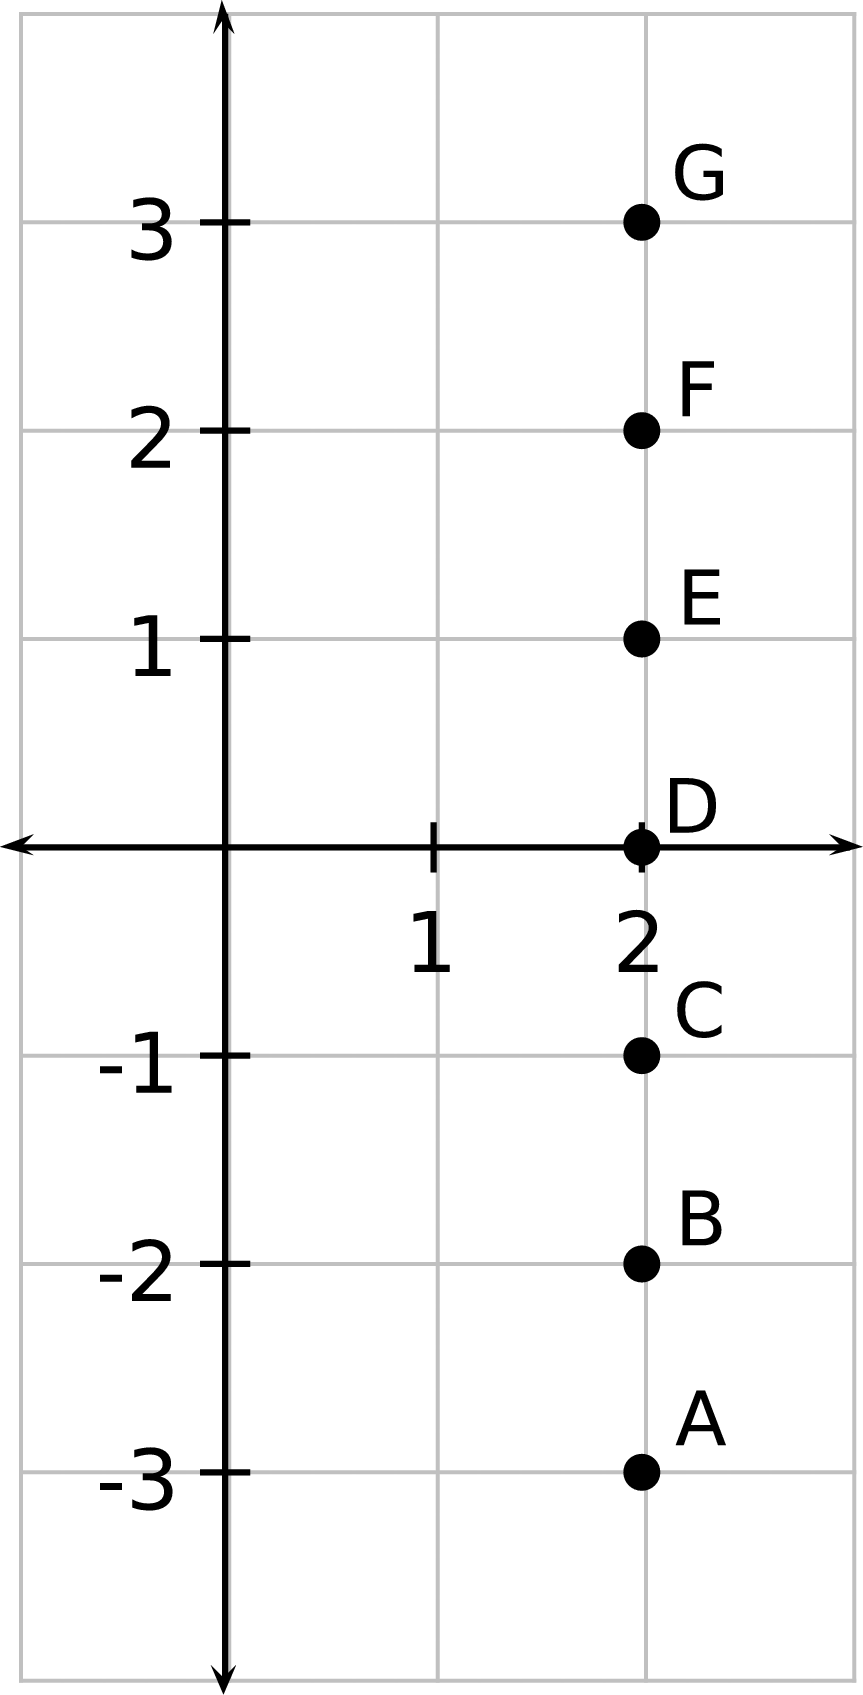
\includegraphics[height=300px]{col11306.imgs/m39358_MG10C14_022.png} % m39358;MG10C14\_022.png;;;6.0;8.5;
%         
%       \vspace{2pt}
%     \vspace{.1in}
%     
%     \end{center}
% 
%  \end{figure}   
% %     
%         \par 
%         
%     % \textbf{m39358*id70156}\par
%     
%           \begin{table}
%         
%     % \begin{table}[H]
%     % \\ '' '0'
%     
%         \begin{center}
%       
%       \label{m39358*id70156}
%       
%     \noindent
%     \tabletail{%
%         \hline
%         \multicolumn{3}{|p{\mytableboxwidth}|}{\raggedleft \small \sl continued on next page}\\
%         \hline
%       }
%       \tablelasttail{}
%       \begin{xtabular}[t]{|l|l|l|}\hline
%     
%     
%         
%                   \textbf{Point}
%                  &
%     
%     
%         
%                   \textbf{$x$ co-ordinate}
%                  &
%     
%     
%         
%                   \textbf{$y$ co-ordinate}
%                 % make-rowspan-placeholders
%      \tabularnewline\cline{1-1}\cline{2-2}\cline{3-3}
%       %--------------------------------------------------------------------
%     
%     
%         A &
%     
%     
%          &
%     
%     
%         % make-rowspan-placeholders
%      \tabularnewline\cline{1-1}\cline{2-2}\cline{3-3}
%       %--------------------------------------------------------------------
%     
%     
%         B &
%     
%     
%          &
%     
%     
%         % make-rowspan-placeholders
%      \tabularnewline\cline{1-1}\cline{2-2}\cline{3-3}
%       %--------------------------------------------------------------------
%     
%     
%         C &
%     
%     
%          &
%     
%     
%         % make-rowspan-placeholders
%      \tabularnewline\cline{1-1}\cline{2-2}\cline{3-3}
%       %--------------------------------------------------------------------
%     
%     
%         D &
%     
%     
%          &
%     
%     
%         % make-rowspan-placeholders
%      \tabularnewline\cline{1-1}\cline{2-2}\cline{3-3}
%       %--------------------------------------------------------------------
%     
%     
%         E &
%     
%     
%          &
%     
%     
%         % make-rowspan-placeholders
%      \tabularnewline\cline{1-1}\cline{2-2}\cline{3-3}
%       %--------------------------------------------------------------------
%     
%     
%         F &
%     
%     
%          &
%     
%     
%         % make-rowspan-placeholders
%      \tabularnewline\cline{1-1}\cline{2-2}\cline{3-3}
%       %--------------------------------------------------------------------
%     
%     
%         G &
%     
%     
%          &
%     
%     
%         % make-rowspan-placeholders
%      \tabularnewline\cline{1-1}\cline{2-2}\cline{3-3}
%       %--------------------------------------------------------------------
%     \end{xtabular}
%       \end{center}
%     \begin{center}{\small\bfseries Table 13.3}\end{center}
%     \begin{caption}{\small\bfseries Table 13.3}\end{caption}
\end{table}
%       
%     \par
%   
%         
%         \label{m39358*id70410}What do you notice about the $x$ co-ordinates? What do you notice about the $y$ co-ordinates?
% What would happen to the co-ordinates of point A, if it was moved to the position of point G?
%  \par 
% 
%         \label{m39358*id70438}When a point is moved vertically up or down on the Cartesian plane, the $x$ co-ordinate of the point remains the same, but the $y$ co-ordinate changes by the amount that the point was moved up or down.\par 
%         \label{m39358*id70461}For example, in  Point A is moved 4 units upwards to the position marked by G. The new $x$ co-ordinate of point A is the same ($x$=1), but the new $y$ co-ordinate is shifted in the positive $y$ direction 4 units and becomes $y$=-2\textbf{+4}=2. The new co-ordinates of point A are therefore G(1;2). Similarly, for point B that is moved downwards by 5 units, the $x$ co-ordinate is the same ($x=-2,5$), but the $y$ co-ordinate is shifted in the negative $y$-direction by 5 units. The new $y$ co-ordinate is therefore $y$=2,5 \textbf{-5}=-2,5.\par 
%         
%     \setcounter{subfigure}{0}
% 
% 
% 	\begin{figure}[H] % horizontal\label{m39358*uid7650}
%     \begin{center}
%     \rule[.1in]{\figurerulewidth}{.005in} \\
%         \label{m39358*uid70!!!underscore!!!media}\label{m39358*uid70!!!underscore!!!printimage}\includegraphics[height=300px]{col11306.imgs/m39358_MG10C14_023.png} % m39358;MG10C14\_023.png;;;6.0;8.5;
%         
%       \vspace{2pt}
%     \vspace{\rubberspace}\par \begin{cnxcaption}
% 	  \small \textbf{Figure 13.42: }Point A is moved 4 units upwards to the position marked by G. Point B is moved 5 units downwards to the position marked by H.
% 	\end{cnxcaption}
%       
%     \vspace{.1in}
%     \rule[.1in]{\figurerulewidth}{.005in} \\
%         
%     \end{center}
% 
%  \end{figure}   
% %     
% \label{m39358*notfhsst!!!underscore!!!id2490}
% \begin{tabular}{cc}
% 	   \hspace*{-50pt}\raisebox{-8 mm}{ \includegraphics[width=0.5in]{col11306.imgs/pstip2.png}  }& 
% 
% 	\begin{minipage}{0.85\textwidth}
% 	\begin{note}
%       {tip: }If a point is shifted upwards, the new $y$ co-ordinate is given by adding the shift to the old $y$ co-ordinate. If a point is shifted downwards, the new $y$ co-ordinate is given by subtracting the shift from the old $y$ co-ordinate.
% 	\end{note}
% 	\end{minipage}
% 	\end{tabular}
% 	\par
%       
% \label{m39358*secfhsst!!!underscore!!!id2491}
%             \subsubsection{  Discussion : Translation of a Point Horizontally }
%             \nopagebreak
%             
%         \label{m39358*id70654}Complete the table, by filling in the co-ordinates of the points shown in the figure.\par 
%         \label{m39358*id70660}
%           
%     \setcounter{subfigure}{0}
% 
% 
% 	\begin{figure}[H] % horizontal\label{m39358*id70663}
%     \begin{center}
%     \label{m39358*id70663!!!underscore!!!media}\label{m39358*id70663!!!underscore!!!printimage}\includegraphics[width=300px]{col11306.imgs/m39358_MG10C14_024.png} % m39358;MG10C14\_024.png;;;6.0;8.5;
%         
%       \vspace{2pt}
%     \vspace{.1in}
%     
%     \end{center}
% 
%  \end{figure}   
% %     
%         \par 
%         
%     % \textbf{m39358*id70670}\par
%     
%           \begin{table}
%         
%     % \begin{table}[H]
%     % \\ '' '0'
%     
%         \begin{center}
%       
%       \label{m39358*id70670}
%       
%     \noindent
%     \tabletail{%
%         \hline
%         \multicolumn{3}{|p{\mytableboxwidth}|}{\raggedleft \small \sl continued on next page}\\
%         \hline
%       }
%       \tablelasttail{}
%       \begin{xtabular}[t]{|l|l|l|}\hline
%     
%     
%         
%                   \textbf{Point}
%                  &
%     
%     
%         
%                   \textbf{$x$ co-ordinate}
%                  &
%     
%     
%         
%                   \textbf{$y$ co-ordinate}
%                 % make-rowspan-placeholders
%      \tabularnewline\cline{1-1}\cline{2-2}\cline{3-3}
%       %--------------------------------------------------------------------
%     
%     
%         A &
%     
%     
%          &
%     
%     
%         % make-rowspan-placeholders
%      \tabularnewline\cline{1-1}\cline{2-2}\cline{3-3}
%       %--------------------------------------------------------------------
%     
%     
%         B &
%     
%     
%          &
%     
%     
%         % make-rowspan-placeholders
%      \tabularnewline\cline{1-1}\cline{2-2}\cline{3-3}
%       %--------------------------------------------------------------------
%     
%     
%         C &
%     
%     
%          &
%     
%     
%         % make-rowspan-placeholders
%      \tabularnewline\cline{1-1}\cline{2-2}\cline{3-3}
%       %--------------------------------------------------------------------
%     
%     
%         D &
%     
%     
%          &
%     
%     
%         % make-rowspan-placeholders
%      \tabularnewline\cline{1-1}\cline{2-2}\cline{3-3}
%       %--------------------------------------------------------------------
%     
%     
%         E &
%     
%     
%          &
%     
%     
%         % make-rowspan-placeholders
%      \tabularnewline\cline{1-1}\cline{2-2}\cline{3-3}
%       %--------------------------------------------------------------------
%     
%     
%         F &
%     
%     
%          &
%     
%     
%         % make-rowspan-placeholders
%      \tabularnewline\cline{1-1}\cline{2-2}\cline{3-3}
%       %--------------------------------------------------------------------
%     
%     
%         G &
%     
%     
%          &
%     
%     
%         % make-rowspan-placeholders
%      \tabularnewline\cline{1-1}\cline{2-2}\cline{3-3}
%       %--------------------------------------------------------------------
%     \end{xtabular}
%       \end{center}
%     \begin{center}{\small\bfseries Table 13.4}\end{center}
%     \begin{caption}{\small\bfseries Table 13.4}\end{caption}
\end{table}
%       
%     \par
%   
%         
%         \label{m39358*id70923}What do you notice about the $x$ co-ordinates? What do you notice about the $y$ co-ordinates?\par 
%         \label{m39358*id70945}What would happen to the co-ordinates of point A, if it was moved to the position of point G?
%  \par 
% 
%         \label{m39358*id70955}When a point is moved horizontally left or right on the Cartesian plane, the $y$ co-ordinate of the point remains the same, but the $x$ co-ordinate changes by the amount that the point was moved left or right.\par 
%         \label{m39358*id70977}For example, in Figure~13.44 Point A is moved 4 units right to the position marked by G. The new $y$ co-ordinate of point A is the same ($y$=1), but the new $x$ co-ordinate is shifted in the positive $x$ direction 4 units and becomes $x$=-2\textbf{+4}=2. The new co-ordinate of point A at G is therefore (2;1). Similarly, for point B that is moved left by 5 units, the $y$ co-ordinate is the same ($y=-2,5$), but the $x$ co-ordinate is shifted in the negative $x$-direction by 5 units. The new $x$ co-ordinate is therefore $x$=2,5 \textbf{-5}=-2,5. The new co-ordinates of point B at H is therefore (-2,5;1).\par 
%         
%     \setcounter{subfigure}{0}
% 
% 
% 	\begin{figure}[H] % horizontal\label{m39358*uid7134}
%     \begin{center}
%     \rule[.1in]{\figurerulewidth}{.005in} \\
%         \label{m39358*uid7134!!!underscore!!!media}\label{m39358*uid71!!!underscore!!!printimage}\includegraphics[width=300px]{col11306.imgs/m39358_MG10C14_025.png} % m39358;MG10C14\_025.png;;;6.0;8.5;
%         
%       \vspace{2pt}
%     \vspace{\rubberspace}\par \begin{cnxcaption}
% 	  \small \textbf{Figure 13.44: }Point A is moved 4 units to the right to the position marked by G. Point B is moved 5 units to the left to the position marked by H.
% 	\end{cnxcaption}
%       
%     \vspace{.1in}
%     \rule[.1in]{\figurerulewidth}{.005in} \\
%         
%     \end{center}
% 
%  \end{figure}   
% %     
% \label{m39358*notfhsst!!!underscore!!!id2567}
% \begin{tabular}{cc}
% 	   \hspace*{-50pt}\raisebox{-8 mm}{ \includegraphics[width=0.5in]{col11306.imgs/pstip2.png}  }& 
% 
% 	\begin{minipage}{0.85\textwidth}
% 	\begin{note}
%       {tip: }If a point is shifted to the right, the new $x$ co-ordinate is given by adding the shift to the old $x$ co-ordinate. If a point is shifted to the left, the new $x$ co-ordinate is given by subtracting the shift from the old $x$ co-ordinate.
% 	\end{note}
% 	\end{minipage}
% 	\end{tabular}
% 	\par
%       
%       
%       \label{m39358*uid7542}
%             \subsubsection{ Reflection of a Point}
%             \nopagebreak
%             
%         
%         \label{m39358*id71174}When you stand in front of a mirror your reflection is located the same distance ($d$) behind the mirror as you are standing in front of the mirror.\par 
%         \label{m39358*id71188}
%           
%     \setcounter{subfigure}{0}
% 
% 
% 	\begin{figure}[H] % horizontal\label{m39358*id71191}
%     \begin{center}
%     \label{m39358*id71191!!!underscore!!!media}\label{m39358*id71191!!!underscore!!!printimage}\includegraphics{col11306.imgs/m39358_MG10C14_026.png} % m39358;MG10C14\_026.png;;;6.0;8.5;
%         
%       \vspace{2pt}
%     \vspace{.1in}
%     
%     \end{center}
% 
%  \end{figure}   
% %     
%         \par 
%         \label{m39358*id71197}We can apply the same idea to a point that is reflected on the $x$-axis, the $y$-axis and the line $y=x$.\par 
%         \label{m39358*uid7354}
%             \subsubsection{ Reflection on the $x$-axis}
%             \nopagebreak
%             
%           
%           \label{m39358*id71251}If a point is reflected on the $x$-axis, then the reflection must be the same distance below the $x$-axis as the point is above the $x$-axis and vice-versa, as though it were a mirror image.\par 
%           
%     \setcounter{subfigure}{0}
% 
% 
% 	\begin{figure}[H] % horizontal\label{m39358*uid7432}
%     \begin{center}
%     \rule[.1in]{\figurerulewidth}{.005in} \\
%         \label{m39358*uid7432!!!underscore!!!media}\label{m39358*uid74!!!underscore!!!printimage}\includegraphics[width=300px]{col11306.imgs/m39358_MG10C14_027.png} % m39358;MG10C14\_027.png;;;6.0;8.5;
%         
%       \vspace{2pt}
%     \vspace{\rubberspace}\par \begin{cnxcaption}
% 	  \small \textbf{Figure 13.46: }Points A and B are reflected on the $x$-axis. The original points are shown with $\ensuremath{\bullet}$ and the reflected points are shown with $\circ $.
% 	\end{cnxcaption}
%       
%     \vspace{.1in}
%     \rule[.1in]{\figurerulewidth}{.005in} \\
%         
%     \end{center}
% 
%  \end{figure}   
% %     
% \label{m39358*notfhsst!!!underscore!!!id2591}
% \begin{tabular}{cc}
% 	   \hspace*{-50pt}\raisebox{-8 mm}{ \includegraphics[width=0.5in]{col11306.imgs/pstip2.png}  }& 
% 
% 	\begin{minipage}{0.85\textwidth}
% 	\begin{note}
%       {tip: }When a point is reflected about the $x$-axis, only the $y$ co-ordinate of the point changes.
% 	\end{note}
% 	\end{minipage}
% 	\end{tabular}
% 	\par
%       
% \label{m39358*secfhsst!!!underscore!!!id2592}\vspace{.5cm} 
%       
%       \noindent
%       \hspace*{-30pt}\includegraphics[width=0.5in]{col11306.imgs/pspencil2.png}   \raisebox{25mm}{   
%       \begin{mdframed}[linewidth=4, leftmargin=40, rightmargin=40]  
%       \begin{exercise}
%     \noindent\textbf{Exercise 13.11:  Reflection on the $x$-axis }
%           \label{m39358*probfhsst!!!underscore!!!id2593}
%           \label{m39358*id71366}Find the co-ordinates of the reflection of the point P, if P is reflected on the $x$-axis. The co-ordinates of P are (5;10). \par 
%           \vspace{5pt}
%           \label{m39358*solfhsst!!!underscore!!!id2596}\noindent\textbf{Solution to Exercise } \label{m39358*listfhsst!!!underscore!!!id2596}\begin{enumerate}[noitemsep, label=\textbf{Step} \textbf{\arabic*}. ] 
%             \leftskip=20pt\rightskip=\leftskip\item  
%           \label{m39358*id71399}We are given the point P with co-ordinates (5;10) and need to find the co-ordinates of the point if it is reflected on the $x$-axis.\par 
%           \item  
%           \label{m39358*id71417}The point P is above the $x$-axis, therefore its reflection will be the same distance below the $x$-axis as the point P is above the $x$-axis. Therefore, $y$=-10.\par 
%           \label{m39358*id71457}For a reflection on the $x$-axis, the $x$ co-ordinate remains unchanged. Therefore, $x$=5.\par 
%           \item  
%           \label{m39358*id71490}The co-ordinates of the reflected point are (5;-10).
%  \par 
%           \end{enumerate}
%          
% 
%     \end{exercise}
%     \end{mdframed}
%     }
%     \noindent
%   
%         
%         \label{m39358*uid765}
%             \subsubsection{ Reflection on the $y$-axis}
%             \nopagebreak
%             
%           
%           \label{m39358*id71525}If a point is reflected on the $y$-axis, then the reflection must be the same distance to the left of the $y$-axis as the point is to the right of the $y$-axis and vice-versa.\par 
%           
%     \setcounter{subfigure}{0}
% 
% 
% 	\begin{figure}[H] % horizontal\label{m39358*uid7645}
%     \begin{center}
%     \rule[.1in]{\figurerulewidth}{.005in} \\
%         \label{m39358*uid7645!!!underscore!!!media}\label{m39358*uid76!!!underscore!!!printimage}\includegraphics[width=300px]{col11306.imgs/m39358_MG10C14_028.png} % m39358;MG10C14\_028.png;;;6.0;8.5;
%         
%       \vspace{2pt}
%     \vspace{\rubberspace}\par \begin{cnxcaption}
% 	  \small \textbf{Figure 13.47: }Points A and B are reflected on the $y$-axis. The original points are shown with $\ensuremath{\bullet}$ and the reflected points are shown with $\circ $.
% 	\end{cnxcaption}
%       
%     \vspace{.1in}
%     \rule[.1in]{\figurerulewidth}{.005in} \\
%         
%     \end{center}
% 
%  \end{figure}   
% %     
% \label{m39358*notfhsst!!!underscore!!!id2618}
% \begin{tabular}{cc}
% 	   \hspace*{-50pt}\raisebox{-8 mm}{ \includegraphics[width=0.5in]{col11306.imgs/pstip2.png}  }& 
% 
% 	\begin{minipage}{0.85\textwidth}
% 	\begin{note}
%       {tip: }When a point is reflected on the $y$-axis, only the $x$ co-ordinate of the point changes. The $y$ co-ordinate remains unchanged.
% 	\end{note}
% 	\end{minipage}
% 	\end{tabular}
% 	\par
%       
% \label{m39358*secfhsst!!!underscore!!!id2619}\vspace{.5cm} 
%       
%       \noindent
%       \hspace*{-30pt}\includegraphics[width=0.5in]{col11306.imgs/pspencil2.png}   \raisebox{25mm}{   
%       \begin{mdframed}[linewidth=4, leftmargin=40, rightmargin=40]  
%       \begin{exercise}
%     \noindent\textbf{Exercise 13.12:  Reflection on the $y$-axis }
%           \label{m39358*probfhsst!!!underscore!!!id2620}
%           \label{m39358*id71649}Find the co-ordinates of the reflection of the point Q, if Q is reflected on the $y$-axis. The co-ordinates of Q are (15;5). \par 
%           \vspace{5pt}
%           \label{m39358*solfhsst!!!underscore!!!id2623}\noindent\textbf{Solution to Exercise } \label{m39358*listfhsst!!!underscore!!!id2623}\begin{enumerate}[noitemsep, label=\textbf{Step} \textbf{\arabic*}. ] 
%             \leftskip=20pt\rightskip=\leftskip\item  
%           \label{m39358*id71682}We are given the point Q with co-ordinates (15;5) and need to find the co-ordinates of the point if it is reflected on the $y$-axis.\par 
%           \item  
%           \label{m39358*id71700}The point Q is to the right of the $y$-axis, therefore its reflection will be the same distance to the left of the $y$-axis as the point Q is to the right of the $y$-axis. Therefore, $x$=-15.\par 
%           \label{m39358*id71740}For a reflection on the $y$-axis, the $y$ co-ordinate remains unchanged. Therefore, $y$=5.\par 
%           \item  
%           \label{m39358*id71774}The co-ordinates of the reflected point are (-15;5).
%  \par 
%           \end{enumerate}
%          
% 
%     \end{exercise}
%     \end{mdframed}
%     }
%     \noindent
%   
%         
%         \label{m39358*uid77754}
%             \subsubsection{ Reflection on the line $y=x$}
%             \nopagebreak
%             
%           
%           \label{m39358*id71812}The final type of reflection you will learn about is the reflection of a point on the line $y=x$.\par 
% \label{m39358*secfhsst!!!underscore!!!id2638}
%             \subsubsection{  Casestudy : Reflection of a point on the line $y=x$ }
%             \nopagebreak
%             
%           \label{m39358*id71852}
%             
%     \setcounter{subfigure}{0}
% 
% 
% 	\begin{figure}[H] % horizontal\label{m39358*id71857}
%     \begin{center}
%     \label{m39358*id71857!!!underscore!!!media}\label{m39358*id71857!!!underscore!!!printimage}\includegraphics[width=300px]{col11306.imgs/m39358_MG10C14_029.png} % m39358;MG10C14\_029.png;;;6.0;8.5;
%         
%       \vspace{2pt}
%     \vspace{.1in}
%     
%     \end{center}
% 
%  \end{figure}   
% %     
%           \par 
%           \label{m39358*id71863}Study the information given and complete the following table:\par 
%           
%     % \textbf{m39358*id71867}\par
%     
%           \begin{table}
%         
%     % \begin{table}[H]
%     % \\ '' '0'
%     
%         \begin{center}
%       
%       \label{m39358*id71867}
%       
%     \noindent
%     \tabletail{%
%         \hline
%         \multicolumn{3}{|p{\mytableboxwidth}|}{\raggedleft \small \sl continued on next page}\\
%         \hline
%       }
%       \tablelasttail{}
%       \begin{xtabular}[t]{|l|l|l|}\hline
%     
%     
%          &
%     
%     
%         
%                     \textbf{Point}
%                    &
%     
%     
%         
%                     \textbf{Reflection}
%                   % make-rowspan-placeholders
%      \tabularnewline\cline{1-1}\cline{2-2}\cline{3-3}
%       %--------------------------------------------------------------------
%     
%     
%         A &
%     
%     
%         (2;1) &
%     
%     
%         (1;2)% make-rowspan-placeholders
%      \tabularnewline\cline{1-1}\cline{2-2}\cline{3-3}
%       %--------------------------------------------------------------------
%     
%     
%         B &
%     
%     
%         (-$1\frac{1}{2}$;-2) &
%     
%     
%         (-2;-1$\frac{1}{2}$)% make-rowspan-placeholders
%      \tabularnewline\cline{1-1}\cline{2-2}\cline{3-3}
%       %--------------------------------------------------------------------
%     
%     
%         C &
%     
%     
%         (-1;1) &
%     
%     
%         % make-rowspan-placeholders
%      \tabularnewline\cline{1-1}\cline{2-2}\cline{3-3}
%       %--------------------------------------------------------------------
%     
%     
%         D &
%     
%     
%         (2;-3) &
%     
%     
%         % make-rowspan-placeholders
%      \tabularnewline\cline{1-1}\cline{2-2}\cline{3-3}
%       %--------------------------------------------------------------------
%     \end{xtabular}
%       \end{center}
%     \begin{center}{\small\bfseries Table 13.5}\end{center}
%     \begin{caption}{\small\bfseries Table 13.5}\end{caption}
\end{table}
%       
%     \par
%   
%           
%           \label{m39358*id72055}What can you deduce about the co-ordinates of points that are reflected about the line $y=x$? \par 
% 
%           \label{m39358*id72080}The $x$ and $y$ co-ordinates of points that are reflected on the line $y=x$ are swapped around, or interchanged. This means that the $x$ co-ordinate of the original point becomes the $y$ co-ordinate of the reflected point and the $y$ co-ordinate of the original point becomes the $x$ co-ordinate of the reflected point.\par 
%           
%     \setcounter{subfigure}{0}
% 
% 
% 	\begin{figure}[H] % horizontal\label{m39358*uid7568}
%     \begin{center}
%     \rule[.1in]{\figurerulewidth}{.005in} \\
%         \label{m39358*uid7568!!!underscore!!!media}\label{m39358*uid7568!!!underscore!!!printimage}\includegraphics[width=300px]{col11306.imgs/m39358_MG10C14_030.png} % m39358;MG10C14\_030.png;;;6.0;8.5;
%         
%       \vspace{2pt}
%     \vspace{\rubberspace}\par \begin{cnxcaption}
% 	  \small \textbf{Figure 13.49: }Points A and B are reflected on the line $y=x$. The original points are shown with $\ensuremath{\bullet}$ and the reflected points are shown with $\circ $.
% 	\end{cnxcaption}
%       
%     \vspace{.1in}
%     \rule[.1in]{\figurerulewidth}{.005in} \\
%         
%     \end{center}
% 
%  \end{figure}   
% %     
% \label{m39358*notfhsst!!!underscore!!!id2694}
% \begin{tabular}{cc}
% 	   \hspace*{-50pt}\raisebox{-8 mm}{ \includegraphics[width=0.5in]{col11306.imgs/pstip2.png}  }& 
% 
% 	\begin{minipage}{0.85\textwidth}
% 	\begin{note}
%       {tip: }The $x$ and $y$ co-ordinates of points that are reflected on the line $y=x$ are interchanged.
% 	\end{note}
% 	\end{minipage}
% 	\end{tabular}
% 	\par
%       
% \label{m39358*secfhsst!!!underscore!!!id2695}\vspace{.5cm} 
%       
%       \noindent
%       \hspace*{-30pt}\includegraphics[width=0.5in]{col11306.imgs/pspencil2.png}   \raisebox{25mm}{   
%       \begin{mdframed}[linewidth=4, leftmargin=40, rightmargin=40]  
%       \begin{exercise}
%     \noindent\textbf{Exercise 13.13:  Reflection on the line $y=x$ }
%           \label{m39358*probfhsst!!!underscore!!!id2696}
%           \label{m39358*id72261}Find the co-ordinates of the reflection of the point R, if R is reflected on the line $y=x$. The co-ordinates of R are (-5;5). \par 
%           \vspace{5pt}
%           \label{m39358*solfhsst!!!underscore!!!id2699}\noindent\textbf{Solution to Exercise } \label{m39358*listfhsst!!!underscore!!!id2699}\begin{enumerate}[noitemsep, label=\textbf{Step} \textbf{\arabic*}. ] 
%             \leftskip=20pt\rightskip=\leftskip\item  
%           \label{m39358*id72300}We are given the point R with co-ordinates (-5;5) and need to find the co-ordinates of the point if it is reflected on the line $y=x$.\par 
%           \item  
%           \label{m39358*id72323}The $x$ co-ordinate of the reflected point is the $y$ co-ordinate of the original point. Therefore, $x$=5.\par 
%           \label{m39358*id72353}The $y$ co-ordinate of the reflected point is the $x$ co-ordinate of the original point. Therefore, $y$=-5.\par 
%           \item  
%           \label{m39358*id72387}The co-ordinates of the reflected point are (5;-5). \par 
%           \end{enumerate}
%          
% 
%     \end{exercise}
%     \end{mdframed}
%     }
%     \noindent
%   
%           \label{m39358*id72402}
%             \uline{Rules of Translation}
%           \par 
%           \label{m39358*id72409}A quick way to write a translation is to use a 'rule of translation'. For example \b \label{m39357*cid3}
%    egin{math}\left(x;y\right)\to \left(x+a;y+b\right)$ means translate point (x;y) by moving a units horizontally and b units vertically.\par 
%           \label{m39358*id72456}So if we translate (1;2) by the rule $\left(x;y\right)\to \left(x+3;y-1\right)$ it becomes (4;1). We have moved 3 units right and 1 unit down.\par 
%           \label{m39358*id72503}
%             \uline{Translating a Region}
%           \par 
%           \label{m39358*id72511}To translate a region, we translate each point in the region.\par 
%           \label{m39358*id72517}
%             \uline{Example}
%           \par 
%           \label{m39358*id72526}Region A has been translated to region B by the rule: $\left(x;y\right)\to \left(x+4;y+2\right)$\par 
%           \label{m39358*id72572}
%             
%     \setcounter{subfigure}{0}
% 
% 
% 	\begin{figure}[H] % horizontal\label{m39358*id72575}
%     \begin{center}
%     \label{m39358*id72575!!!underscore!!!media}\label{m39358*id72575!!!underscore!!!printimage}\includegraphics[width=300px]{col11306.imgs/m39358_MG10C14_031.png} % m39358;MG10C14\_031.png;;;6.0;8.5;
%         
%       \vspace{2pt}
%     \vspace{.1in}
%     
%     \end{center}
% 
%  \end{figure}   
% %     
%           \par 
% \label{m39358*secfhsst!!!underscore!!!id2730}
%             \subsubsection{  Discussion : Rules of Transformations }
%             \nopagebreak
%             
%           \label{m39358*id72588}Work with a friend and decide which item from column 1 matches each description in column 2.\par 
%           
%     % \textbf{m39358*id72595}\par
%     
%           \begin{table}
%         
%     % \begin{table}[H]
%     % \\ '' '0'
%     
%         \begin{center}
%       
%       \label{m39358*id72595}
%       
%     \noindent
%     \tabletail{%
%         \hline
%         \multicolumn{2}{|p{\mytableboxwidth}|}{\raggedleft \small \sl continued on next page}\\
%         \hline
%       }
%       \tablelasttail{}
%       \begin{xtabular}[t]{|l|l|}\hline
%     
%     
%         
%                     \textbf{Column 1}
%                    &
%     
%     
%         
%                     \textbf{Column 2}
%                   % make-rowspan-placeholders
%      \tabularnewline\cline{1-1}\cline{2-2}
%       %--------------------------------------------------------------------
%     
%     
%         1.$\left(x;y\right)\to \left(x;y-3\right)$        &
%     
%     
%         A. a reflection on x-y line% make-rowspan-placeholders
%      \tabularnewline\cline{1-1}\cline{2-2}
%       %--------------------------------------------------------------------
%     
%     
%         2.
%                     $\left(x;y\right)\to \left(x-3;y\right)$
%                    &
%     
%     
%         B. a reflection on the x axis% make-rowspan-placeholders
%      \tabularnewline\cline{1-1}\cline{2-2}
%       %--------------------------------------------------------------------
%     
%     
%         3.
%                     $\left(x;y\right)\to \left(x;-y\right)$
%                    &
%     
%     
%         C. a shift of 3 units left% make-rowspan-placeholders
%      \tabularnewline\cline{1-1}\cline{2-2}
%       %--------------------------------------------------------------------
%     
%     
%         4.
%                     $\left(x;y\right)\to \left(-x;y\right)$
%                    &
%     
%     
%         D. a shift of 3 units down% make-rowspan-placeholders
%      \tabularnewline\cline{1-1}\cline{2-2}
%       %--------------------------------------------------------------------
%     
%     
%         
% 5.
%                     $\left(x;y\right)\to \left(y;x\right)$
%                    &
%     
%     
%         E. a reflection on the y-axis% make-rowspan-placeholders
%      \tabularnewline\cline{1-1}\cline{2-2}
%       %--------------------------------------------------------------------
%     \end{xtabular}
%       \end{center}
%     \begin{center}{\small\bfseries Table 13.6}\end{center}
%     \begin{caption}{\small\bfseries Table 13.6}\end{caption}
\end{table}
%       
%     \par
%   
%   raggedleft \small \sl continued on next page}\\
%         \hline
%       }
%       \tablelasttail{}
%       \begin{xtabular*}{\mytablewidth}[t]{|p{10\mystarwidth}|p{10\mystarwidth}|}\hline
%     % count in rowspan-info-nodeset: 2
%     % align/colidx: left,1
%     
%     % rowcount: '0' | start: 'false' | colidx: '1'
%     
%         % Formatting a regular cell and recurring on the next sibling
%         
%                     \textbf{Column 1}
%                    &
%       % align/colidx: left,2
%     
%     % rowcount: '0' | start: 'false' | colidx: '2'
%     
%         % Formatting a regular cell and recurring on the next sibling
%         
%                     \textbf{Column 2}
%                   % make-rowspan-placeholders
%     % rowspan info: col1 '0' | 'false' | '' || col2 '0' | 'false' | ''
%      \tabularnewline\cline{1-1}\cline{2-2}
%       %--------------------------------------------------------------------
%     % align/colidx: left,1
%     
%     % rowcount: '0' | start: 'false' | colidx: '1'
%     
%         % Formatting a regular cell and recurring on the next sibling
%         1.$\left(x;y\right)\to \left(x;y-3\right)$        &
%       % align/colidx: left,2
%     
%     % rowcount: '0' | start: 'false' | colidx: '2'
%     
%         % Formatting a regular cell and recurring on the next sibling
%         A. a reflection on x-y line% make-rowspan-placeholders
%     % rowspan info: col1 '0' | 'false' | '' || col2 '0' | 'false' | ''
%      \tabularnewline\cline{1-1}\cline{2-2}
%       %--------------------------------------------------------------------
%     % align/colidx: left,1
%     
%     % rowcount: '0' | start: 'false' | colidx: '1'
%     
%         % Formatting a regular cell and recurring on the next sibling
%         2.
%                     $\left(x;y\right)\to \left(x-3;y\right)$
%                    &
%       % align/colidx: left,2
%     
%     % rowcount: '0' | start: 'false' | colidx: '2'
%     
%         % Formatting a regular cell and recurring on the next sibling
%         B. a reflection on the x axis% make-rowspan-placeholders
%     % rowspan info: col1 '0' | 'false' | '' || col2 '0' | 'false' | ''
%      \tabularnewline\cline{1-1}\cline{2-2}
%       %--------------------------------------------------------------------
%     % align/colidx: left,1
%     
%     % rowcount: '0' | start: 'false' | colidx: '1'
%     
%         % Formatting a regular cell and recurring on the next sibling
%         3.
%                     $\left(x;y\right)\to \left(x;-y\right)$
%                    &
%       % align/colidx: left,2
%     
%     % rowcount: '0' | start: 'false' | colidx: '2'
%     
%         % Formatting a regular cell and recurring on the next sibling
%         C. a shift of 3 units left% make-rowspan-placeholders
%     % rowspan info: col1 '0' | 'false' | '' || col2 '0' | 'false' | ''
%      \tabularnewline\cline{1-1}\cline{2-2}
%       %--------------------------------------------------------------------
%     % align/colidx: left,1
%     
%     % rowcount: '0' | start: 'false' | colidx: '1'
%     
%         % Formatting a regular cell and recurring on the next sibling
%         4.
%                     $\left(x;y\right)\to \left(-x;y\right)$
%                    &
%       % align/colidx: left,2
%     
%     % rowcount: '0' | start: 'false' | colidx: '2'
%     
%         % Formatting a regular cell and recurring on the next sibling
%         D. a shift of 3 units down% make-rowspan-placeholders
%     % rowspan info: col1 '0' | 'false' | '' || col2 '0' | 'false' | ''
%      \tabularnewline\cline{1-1}\cline{2-2}
%       %--------------------------------------------------------------------
%     % align/colidx: left,1
%     
%     % rowcount: '0' | start: 'false' | colidx: '1'
%     
%         % Formatting a regular cell and recurring on the next sibling
%         
% 5.
%                     $\left(x;y\right)\to \left(y;x\right)$
%                    &
%       % align/colidx: left,2
%     
%     % rowcount: '0' | start: 'false' | colidx: '2'
%     
%         % Formatting a regular cell and recurring on the next sibling
%         E. a reflection on the y-axis% make-rowspan-placeholders
%     % rowspan info: col1 '0' | 'false' | '' || col2 '0' | 'false' | ''
%      \tabularnewline\cline{1-1}\cline{2-2}
%       %--------------------------------------------------------------------
%     \end{xtabular*}
%       \end{center}
%     \begin{center}{\small\bfseries Table 13.6}\end{center}
%     %\end{table}
%     %     
%         }% ending lr/para test clause
%       
%     \par
%   
%   
%                     $\left(x;y\right)\to \left(x-3;y\right)$
%                    &
%       % align/colidx: left,2
%     
%     % rowcount: '0' | start: 'false' | colidx: '2'
%     
%         % Formatting a regular cell and recurring on the next sibling
%         B. a reflection on the x axis% make-rowspan-placeholders
%     % rowspan info: col1 '0' | 'false' | '' || col2 '0' | 'false' | ''
%      \tabularnewline\cline{1-1}\cline{2-2}
%       %--------------------------------------------------------------------
%     % align/colidx: left,1
%     
%     % rowcount: '0' | start: 'false' | colidx: '1'
%     
%         % Formatting a regular cell and recurring on the next sibling
%         3.
%                     $\left(x;y\right)\to \left(x;-y\right)$
%                    &
%       % align/colidx: left,2
%     
%     % rowcount: '0' | start: 'false' | colidx: '2'
%     
%         % Formatting a regular cell and recurring on the next sibling
%         C. a shift of 3 units left% make-rowspan-placeholders
%     % rowspan info: col1 '0' | 'false' | '' || col2 '0' | 'false' | ''
%      \tabularnewline\cline{1-1}\cline{2-2}
%       %--------------------------------------------------------------------
%     % align/colidx: left,1
%     
%     % rowcount: '0' | start: 'false' | colidx: '1'
%     
%         % Formatting a regular cell and recurring on the next sibling
%         4.
%                     $\left(x;y\right)\to \left(-x;y\right)$
%                    &
%       % align/colidx: left,2
%     
%     % rowcount: '0' | start: 'false' | colidx: '2'
%     
%         % Formatting a regular cell and recurring on the next sibling
%         D. a shift of 3 units down% make-rowspan-placeholders
%     % rowspan info: col1 '0' | 'false' | '' || col2 '0' | 'false' | ''
%      \tabularnewline\cline{1-1}\cline{2-2}
%       %--------------------------------------------------------------------
%     % align/colidx: left,1
%     
%     % rowcount: '0' | start: 'false' | colidx: '1'
%     
%         % Formatting a regular cell and recurring on the next sibling
%         
% 5.
%                     $\left(x;y\right)\to \left(y;x\right)$
%                    &
%       % align/colidx: left,2
%     
%     % rowcount: '0' | start: 'false' | colidx: '2'
%     
%         % Formatting a regular cell and recurring on the next sibling
%         E. a reflection on the y-axis% make-rowspan-placeholders
%     % rowspan info: col1 '0' | 'false' | '' || col2 '0' | 'false' | ''
%      \tabularnewline\cline{1-1}\cline{2-2}
%       %--------------------------------------------------------------------
%     \end{xtabular*}
%       \end{center}
%     \begin{center}{\small\bfseries Table 13.6}\end{center}
%     %\end{table}
%     %     
%         }% ending lr/para test clause
%       
%     \par
%   
%   alse' | '' || col2 '0' | 'false' | ''
%      \tabularnewline\cline{1-1}\cline{2-2}
%       %--------------------------------------------------------------------
%     \end{tabular*}} % end mytableboxdepth set
%         \addtolength{\mytableboxheight}{\mytableboxdepth}
%         % ----- End capturing height of table
%         \typeout{textheight: \the\textheight}
%         \typeout{mytableboxheight: \the\mytableboxheight}
%         \typeout{table too wide, outputting in para mode}
%         
%     % \begin{table}[H]
%     % \\ '' '0'
%     
%         \begin{center}
%       
%       \label{m39358*id72595}
%       
%     \noindent
%     \tabletail{%
%         \hline
%         \multicolumn{2}{|p{\mytableroom}|}{\raggedleft \small \sl continued on next page}\\
%         \hline
%       }
%       \tablelasttail{}
%       \begin{xtabular*}{\mytablewidth}[t]{|p{10\mystarwidth}|p{10\mystarwidth}|}\hline
%     % count in rowspan-info-nodeset: 2
%     % align/colidx: left,1
%     
%     % rowcount: '0' | start: 'false' | colidx: '1'
%     
%         % Formatting a regular cell and recurring on the next sibling
%         
%                     \textbf{Column 1}
%                    &
%       % align/colidx: left,2
%     
%     % rowcount: '0' | start: 'false' | colidx: '2'
%     
%         % Formatting a regular cell and recurring on the next sibling
%         
%                     \textbf{Column 2}
%                   % make-rowspan-placeholders
%     % rowspan info: col1 '0' | 'false' | '' || col2 '0' | 'false' | ''
%      \tabularnewline\cline{1-1}\cline{2-2}
%       %--------------------------------------------------------------------
%     % align/colidx: left,1
%     
%     % rowcount: '0' | start: 'false' | colidx: '1'
%     
%         % Formatting a regular cell and recurring on the next sibling
%         1.$\left(x;y\right)\to \left(x;y-3\right)$        &
%       % align/colidx: left,2
%     
%     % rowcount: '0' | start: 'false' | colidx: '2'
%     
%         % Formatting a regular cell and recurring on the next sibling
%         A. a reflection on x-y line% make-rowspan-placeholders
%     % rowspan info: col1 '0' | 'false' | '' || col2 '0' | 'false' | ''
%      \tabularnewline\cline{1-1}\cline{2-2}
%       %--------------------------------------------------------------------
%     % align/colidx: left,1
%     
%     % rowcount: '0' | start: 'false' | colidx: '1'
%     
%         % Formatting a regular cell and recurring on the next sibling
%         2.
%                     $\left(x;y\right)\to \left(x-3;y\right)$
%                    &
%       % align/colidx: left,2
%     
%     % rowcount: '0' | start: 'false' | colidx: '2'
%     
%         % Formatting a regular cell and recurring on the next sibling
%         B. a reflection on the x axis% make-rowspan-placeholders
%     % rowspan info: col1 '0' | 'false' | '' || col2 '0' | 'false' | ''
%      \tabularnewline\cline{1-1}\cline{2-2}
%       %--------------------------------------------------------------------
%     % align/colidx: left,1
%     
%     % rowcount: '0' | start: 'false' | colidx: '1'
%     
%         % Formatting a regular cell and recurring on the next sibling
%         3.
%                     $\left(x;y\right)\to \left(x;-y\right)$
%                    &
%       % align/colidx: left,2
%     
%     % rowcount: '0' | start: 'false' | colidx: '2'
%     
%         % Formatting a regular cell and recurring on the next sibling
%         C. a shift of 3 units left% make-rowspan-placeholders
%     % rowspan info: col1 '0' | 'false' | '' || col2 '0' | 'false' | ''
%      \tabularnewline\cline{1-1}\cline{2-2}
%       %--------------------------------------------------------------------
%     % align/colidx: left,1
%     
%     % rowcount: '0' | start: 'false' | colidx: '1'
%     
%         % Formatting a regular cell and recurring on the next sibling
%         4.
%                     $\left(x;y\right)\to \left(-x;y\right)$
%                    &
%       % align/colidx: left,2
%     
%     % rowcount: '0' | start: 'false' | colidx: '2'
%     
%         % Formatting a regular cell and recurring on the next sibling
%         D. a shift of 3 units down% make-rowspan-placeholders
%     % rowspan info: col1 '0' | 'false' | '' || col2 '0' | 'false' | ''
%      \tabularnewline\cline{1-1}\cline{2-2}
%       %--------------------------------------------------------------------
%     % align/colidx: left,1
%     
%     % rowcount: '0' | start: 'false' | colidx: '1'
%     
%         % Formatting a regular cell and recurring on the next sibling
%         
% 5.
%                     $\left(x;y\right)\to \left(y;x\right)$
%                    &
%       % align/colidx: left,2
%     
%     % rowcount: '0' | start: 'false' | colidx: '2'
%     
%         % Formatting a regular cell and recurring on the next sibling
%         E. a reflection on the y-axis% make-rowspan-placeholders
%     % rowspan info: col1 '0' | 'false' | '' || col2 '0' | 'false' | ''
%      \tabularnewline\cline{1-1}\cline{2-2}
%       %--------------------------------------------------------------------
%     \end{xtabular*}
%       \end{center}
%     \begin{center}{\small\bfseries Table 13.6}\end{center}
%     %\end{table}
%     %     
%         }% ending lr/para test clause
%       
%     \par
%   
%           
%           
% 
% \label{m39358*secfhsst!!!underscore!!!id2841}
%             \subsubsection{  Transformations }
%             \nopagebreak
%             
%           \label{m39358*id72872}\begin{enumerate}[noitemsep, label=\textbf{\arabic*}. ] 
%             \label{m39358*uid76349}\item Describe the translations in each of the following using the rule (x;y)$\to $ (...;...)
% 
%     \setcounter{subfigure}{0}
% 
% 
% 	\begin{figure}[H] % horizontal\label{m39358*id72951}
%     \begin{center}
%     \label{m39358*id72951!!!underscore!!!media}\label{m39358*id72951!!!underscore!!!printimage}\includegraphics[height=300px]{col11306.imgs/m39358_mg10c14_4.png} % m39358;mg10c14\_4.png;;;6.0;8.5;
%         
%       \vspace{2pt}
%     \vspace{.1in}
%     
%     \end{center}
% 
%  \end{figure}   
% %     
% \label{m39358*id72888}\begin{enumerate}[noitemsep, label=\textbf{\alph*}. ] 
%             \label{m39358*uid890}\item From A to B
% \label{m39358*uid891}\item From C to J
% \label{m39358*uid892}\item From F to H
% \label{m39358*uid893}\item From I to J
% \label{m39358*uid8931}\item From K to L
% \label{m39358*uid8932}\item From J to E
% \label{m39358*uid8933}\item From G to H
% \end{enumerate}
%                 \label{m39358*uid874}\item A is the point (4;1).  Plot each of the following points under the given transformations. Give the co-ordinates of the points you have plotted.
% \label{m39358*id72970}\begin{enumerate}[noitemsep, label=\textbf{\alph*}. ] 
%             \label{m39358*uid875}\item B is the reflection of A in the x-axis.
% \label{m39358*uid876}\item C is the reflection of A in the y-axis.
% \label{m39358*uid877}\item D is the reflection of B in the line x=0.
% \label{m39358*uid878}\item E is the reflection of C is the line y=0.
% \label{m39358*uid879}\item F is the reflection of A in the line y= x
% \end{enumerate}
%                 \label{m39358*uid970}\item 
%               In the diagram, B, C and D are images of polygon A.  In each case, the transformation that has been applied to obtain the image involves a reflection and a translation of A.  Write down the letter of each image and describe the transformation applied to A in order to obtain the image.
% 
%     \setcounter{subfigure}{0}
% 
% 
% 	\begin{figure}[H] % horizontal\label{m39358*id7327723}
%     \begin{center}
%     \label{m39358*id7327723!!!underscore!!!media}\label{m39358*id7327723!!!underscore!!!printimage}\includegraphics[width=300px]{col11306.imgs/m39358_mg10c14_5.png} % m39358;mg10c14\_5.png;;;6.0;8.5;
%         
%       \vspace{2pt}
%     \vspace{.1in}
%     
%     \end{center}
% 
%  \end{figure}   
% %     
%         
%             \end{enumerate}
%         
%           
% 
% \label{m39358*secfhsst!!!underscore!!!id2877}
% \par \raisebox{-5 pt}{\includegraphics[width=0.5cm]{col11306.imgs/summary_www.png}} Find the answers with the shortcodes:
%  \par \begin{tabular}[h]{cccccc}
%  (1.) laC  &  (2.) la1  &  (3.) lar  & \end{tabular}
% 
% 
% 
%             \subsubsection{  Investigation : Calculation of Volume, Surface Area and scale factors of objects }
%             \nopagebreak
%             
%           \label{m39358*id73612}\begin{enumerate}[noitemsep, label=\textbf{\arabic*}. ] 
%             \label{m39358*uid106}\item Look around the house or school and find a can or a tin of any kind (e.g. beans, soup, cooldrink, paint etc.)
% \label{m39358*uid107}\item Measure the height of the tin and the diameter of its top or bottom.
% \label{m39358*uid108}\item Write down the values you measured on the diagram below:
% 
%     \setcounter{subfigure}{0}
% 
% 
% 	\begin{figure}[H] % horizontal\label{m39358*id73656}
%     \begin{center}
%     \label{m39358*id73656!!!underscore!!!media}\label{m39358*id73656!!!underscore!!!printimage}\includegraphics[width=300px]{col11306.imgs/m39358_MG10C14_034.png} % m39358;MG10C14\_034.png;;;6.0;8.5;
%         
%       \vspace{2pt}
%     \vspace{.1in}
%     
%     \end{center}
% 
%  \end{figure}   
% %     \label{m39358*uid109}\item Using your measurements, calculate the following (in cm${}^{2}$, rounded off to 2 decimal places):
% \label{m39358*id73690}\begin{enumerate}[noitemsep, label=\textbf{\alph*}. ] 
%             \label{m39358*uid110}\item the area of the side of the tin (i.e. the rectangle)
% \label{m39358*uid111}\item the area of the top and bottom of the tin (i.e. the circles)
% \label{m39358*uid112}\item the total surface area of the tin
% \end{enumerate}
%         \label{m39358*uid113}\item If the tin metal costs 0,17 cents/cm${}^{2}$, how much does it cost to make the tin?
% \label{m39358*uid114}\item Find the volume of your tin (in cm${}^{3}$, rounded off to 2 decimal places).
% \label{m39358*uid115}\item What is the volume of the tin given on its label?
% \label{m39358*uid116}\item Compare the volume you calculated with the value given on the label. How much air is contained in the tin when it contains the product (i.e. cooldrink, soup etc.)
% \label{m39358*uid117}\item Why do you think space is left for air in the tin?
% \label{m39358*uid118}\item If you wanted to double the volume of the tin, but keep the radius the same, by how much would you need to increase the height?
% \label{m39358*uid119}\item If the height of the tin is kept the same, but now the radius is doubled, by what scale factor will the:
% \label{m39358*id73845}\begin{enumerate}[noitemsep, label=\textbf{\alph*}. ] 
%             \label{m39358*uid120}\item area of the side surface of the tin increase?
% \label{m39358*uid121}\item area of the bottom/top of the tin increase?
% \end{enumerate}
%         \end{enumerate}
%         
%           
% 
%         
    \label{m39358*eip-803}
            \subsection{ Summary}
            \nopagebreak
            \label{m39358*eip-241}\begin{itemize}[noitemsep]
            \item The properties of kites, rhombuses, parallelograms, squares, rectangles and trapeziums was covered. These figures are all known as quadrilaterals\item You should know the formulae for surface area of rectangular and triangular prisms as well as cylinders\item 
The volume of a right prism is calculated by multiplying the area of the base by the height. So, for a square prism of side length $a$ and height $h$ the volume is $a\ensuremath{\times}a\ensuremath{\times}h={a}^{2}h$.\item 
 Two polygons are similar if:\label{m39358*id938472}\begin{itemize}[noitemsep]
            \item their corresponding angles are equal\item the ratios of corresponding sides are equal\end{itemize}
        . All squares are similar\end{itemize}
        \label{m39358*cid7}
            \subsection{ End of Chapter Exercises}
            \nopagebreak
      \label{m39358*id73895}\begin{enumerate}[noitemsep, label=\textbf{\arabic*}. ] 
            \label{m39358*uid225}\item Assess whether the following statements are true or false. If the statement is false, explain why:
\label{m39358*id73912}\begin{enumerate}[noitemsep, label=\textbf{\alph*}. ] 
            \item  A trapezium is a quadrilateral with two pairs of parallel opposite sides.\item  Both diagonals of a parallelogram bisect each other.\item  A rectangle is a parallelogram that has all four corner angles equal to 60\ensuremath{{\,}^{\circ}}.\item  The four sides of a rhombus have different lengths.\item  The diagonals of a kite intersect at right angles.\item  Two polygons are similar if only their corresponding angles are equal.\end{enumerate}
                \label{m39358*uid1219}\item Calculate the area of each of the following shapes:
    \setcounter{subfigure}{0}
	\begin{figure}[H] % horizontal\label{m39358*id320600}
    \begin{center}
    \label{m39358*id320600!!!underscore!!!media}\label{m39358*id320600!!!underscore!!!printimage}\includegraphics[height=300px]{col11306.imgs/m39358_MG10C14_041.png} % m39358;MG10C14\_041.png;;;6.0;8.5;
      \vspace{2pt}
    \vspace{.1in}
    \end{center}
 \end{figure}               \label{m39358*uid1217}\item Calculate the surface area and volume of each of the following objects (assume that all faces/surfaces are solid -- e.g. surface area of cylinder will include circular areas at top and bottom):
    \setcounter{subfigure}{0}
	\begin{figure}[H] % horizontal\label{m39358*id320601}
    \begin{center}
    \label{m39358*id320601!!!underscore!!!media}\label{m39358*id320601!!!underscore!!!printimage}\includegraphics[width=300px]{col11306.imgs/m39358_MG10C14_042.png} % m39358;MG10C14\_042.png;;;6.0;8.5;
      \vspace{2pt}
    \vspace{.1in}
    \end{center}
 \end{figure}               \label{m39358*uid1218}\item Calculate the surface area and volume of each of the following objects (assume that all faces/surfaces are solid):
    \setcounter{subfigure}{0}
	\begin{figure}[H] % horizontal\label{m39358*id320602}
    \begin{center}
    \label{m39358*id320602!!!underscore!!!media}\label{m39358*id320602!!!underscore!!!printimage}\includegraphics[height=300px]{col11306.imgs/m39358_MG10C14_043.png} % m39358;MG10C14\_043.png;;;6.0;8.5;
      \vspace{2pt}
    \vspace{.1in}
    \end{center}
 \end{figure}               \label{m39358*uid125}\item Using the rules given, identify the type of transformation and draw the image of the shapes.
\label{m39358*id73963}\begin{enumerate}[noitemsep, label=\textbf{\alph*}. ] 
            \label{m39358*uid126}\item  (x;y)$\to $(x+3;y-3)
    \setcounter{subfigure}{0}
	\begin{figure}[H] % horizontal\label{m39358*id73991}
    \begin{center}
    \label{m39358*id73991!!!underscore!!!media}\label{m39358*id73991!!!underscore!!!printimage}\includegraphics[width=300px]{col11306.imgs/m39358_MG10C14_037.png} % m39358;MG10C14\_037.png;;;6.0;8.5;
      \vspace{2pt}
    \vspace{.1in}
    \end{center}
 \end{figure}       \label{m39358*uid127}\item  (x;y)$\to $(x-4;y)
    \setcounter{subfigure}{0}
	\begin{figure}[H] % horizontal\label{m39358*id74022}
    \begin{center}
    \label{m39358*id74022!!!underscore!!!media}\label{m39358*id74022!!!underscore!!!printimage}\includegraphics[width=300px]{col11306.imgs/m39358_MG10C14_038.png} % m39358;MG10C14\_038.png;;;6.0;8.5;
      \vspace{2pt}
    \vspace{.1in}
    \end{center}
 \end{figure}       \label{m39358*uid128}\item (x;y)$\to $(y;x)
    \setcounter{subfigure}{0}
	\begin{figure}[H] % horizontal\label{m39358*id74053}
    \begin{center}
    \label{m39358*id74053!!!underscore!!!media}\label{m39358*id74053!!!underscore!!!printimage}\includegraphics[width=300px]{col11306.imgs/m39358_MG10C14_039.png} % m39358;MG10C14\_039.png;;;6.0;8.5;
      \vspace{2pt}
    \vspace{.1in}
    \end{center}
 \end{figure}       \label{m39358*uid129}\item (x;y)$\to $(-x;-y)
    \setcounter{subfigure}{0}
	\begin{figure}[H] % horizontal\label{m39358*id74084}
    \begin{center}
    \label{m39358*id74084!!!underscore!!!media}\label{m39358*id74084!!!underscore!!!printimage}\includegraphics[width=300px]{col11306.imgs/m39358_MG10C14_040.png} % m39358;MG10C14\_040.png;;;6.0;8.5;
      \vspace{2pt}
    \vspace{.1in}
    \end{center}
 \end{figure}       \end{enumerate}
                \item  
PQRS is a quadrilateral with points P(0; −3) ; Q(−2;5) ; R(3;2) and S(3;--2)  in the Cartesian plane.
\label{m39358*id0812312}\begin{enumerate}[noitemsep, label=\textbf{\alph*}. ] 
            \label{m39358*id08123}\item Find the length of QR.\label{m39358*id981221}\item Find the gradient of PS.\label{m39358*id08213}\item Find the midpoint of PR.\label{m39358*id9871293}\item Is PQRS a parallelogram?  Give reasons for your answer. \end{enumerate}
                \item A(--2;3) and B(2;6) are points in the Cartesian plane.  C(a;b) is the midpoint of AB. Find the values of a and b.\newline
\item 
Consider: Triangle ABC with vertices A (1; 3) B (4; 1) and C (6; 4):
\label{m39358*id9173123}\begin{enumerate}[noitemsep, label=\textbf{\alph*}. ] 
            \item Sketch triangle ABC on the Cartesian plane. \item Show that ABC is an isoceles triangle.\item Determine the co-ordinates of M, the midpoint of AC.\item Determine the gradient of AB.\item Show that the following points are collinear: A, B and D(7;-1)\end{enumerate}
\item In the diagram, A is the point (-6;1) and B is the point (0;3)
    \setcounter{subfigure}{0}
	\begin{figure}[H] % horizontal\label{m39358*id740344}
    \begin{center}
    \label{m39358*id740344!!!underscore!!!media}\label{m39358*id740344!!!underscore!!!printimage}\includegraphics[width=.7\columnwidth]{col11306.imgs/m39358_MG10C14_5.png} % m39358;MG10C14\_5.png;;;6.0;8.5;
      \vspace{2pt}
    \vspace{.1in}
    \end{center}
 \end{figure}       \label{m39358*id982373}\begin{enumerate}[noitemsep, label=\textbf{\alph*}. ] 
            \item Find the equation of line AB \item Calculate the length of AB\item  A' is the image of A and B' is the image of B. Both these images are obtain by applying the transformation: (x;y)$\to $(x-4;y-1). Give the coordinates of both A' and B'\item Find the equation of A'B'\item Calculate the length of A'B'\item Can you state with certainty that AA'B'B is a parallelogram? Justify your answer.\end{enumerate}
                 \item The vertices of triangle PQR have co-ordinates as shown in the diagram.
    \setcounter{subfigure}{0}
	\begin{figure}[H] % horizontal\label{m39358*id743344}
    \begin{center}
    \label{m39358*id743344!!!underscore!!!media}\label{m39358*id743344!!!underscore!!!printimage}\includegraphics[width=300px]{col11306.imgs/m39358_mg10c14_6.png} % m39358;mg10c14\_6.png;;;6.0;8.5;
      \vspace{2pt}
    \vspace{.1in}
    \end{center}
 \end{figure}       
\label{m39358*id982372432}\begin{enumerate}[noitemsep, label=\textbf{\alph*}. ] 
            \item Give the co-ordinates of  P', Q' and R', the images of P, Q and R when P, Q and R are reflected in the line y=x.\item Determine the area of triangle PQR.\end{enumerate}
\label{m39358*uid1206}\item Which of the following claims are true? Give a counter-example for those that are incorrect.
\label{m39358*id320334}\begin{enumerate}[noitemsep, label=\textbf{\alph*}. ] 
            \label{m39358*uid1216}\item All equilateral triangles are similar.
\label{m39358*uid1226}\item All regular quadrilaterals are similar.
\label{m39358*uid1236}\item In any $▵ABC$\hspace{1ex} with $\angle ABC={90}^{\circ }$ we have $A{B}^{3}+B{C}^{3}=C{A}^{3}$.
\label{m39358*uid1246}\item All right-angled isosceles triangles with perimeter 10 cm are congruent.
\label{m39358*uid1256}\item All rectangles with the same area are similar.
\end{enumerate}
\label{m39358*uid1316}\item For each pair of figures state whether they are similar or not. Give reasons.
    \setcounter{subfigure}{0}
	\begin{figure}[H] % horizontal\label{m39358*id320590}
    \begin{center}
    \label{m39358*id320590!!!underscore!!!media}\label{m39358*id320590!!!underscore!!!printimage}\includegraphics[width=.8\columnwidth]{col11306.imgs/m39358_MG10C13_053.png} % m39358;MG10C13\_053.png;;;6.0;8.5;
      \vspace{2pt}
    \vspace{.1in}
    \end{center}
 \end{figure}               \end{enumerate}
  \label{m39358**end}
  \label{84e7e983e7dc2060d6909eddb5375c22**end}
\par \raisebox{-5 pt}{\includegraphics[width=0.5cm]{col11306.imgs/summary_www.png}} Find the answers with the shortcodes:
 \par \begin{tabular}[h]{cccccc}
 (1.) lbr  &  (2.) lT9  &  (3.) lTX  &  (4.) lTI  &  (5.) la7  &  (6.) laY  &  (7.) laq  &  (8.) la4  &  (9.) l4o  &  (10.) laG  &  (11.) lal  &  (12.) la3  & \end{tabular}
    \label{m39368*eip-514}
            \subsection{ Summary}
            \nopagebreak
            \label{m39368*eip-439}\begin{itemize}[noitemsep]
            \item Make sure you know what the following terms mean: quadrilaterals, vertices, sides, angles, parallel lines, perpendicular lines,diagonals, bisectors and transversals.\item The properties of triangles has been covered.\item Congruency and similarity of triangles\item Angles can be classified as acute, right, obtuse, straight, reflex or revolution\item Theorem of Pythagoras which is used to calculate the lengths of sides of a right-angled triangle\item Angles: \label{m39368*id98732}\begin{itemize}[noitemsep]
            \item Acute angle: An angle ${0}^{\circ }$ and ${90}^{\circ }$\item Right angle: An angle measuring ${90}^{\circ }$\item Obtuse angle: An angle ${90}^{\circ }$ and ${180}^{\circ }$\item Straight angle: An angle measuring ${180}^{\circ }$\item Reflex angle: An angle ${180}^{\circ }$ and ${360}^{\circ }$\item Revolution: An angle measuring ${360}^{\circ }$\end{itemize}
        \item There are several properties of angles and some special names for these\item There are four types of triangles: Equilateral, isoceles, right-angled and scalene\item The angles in a triangle add up to ${180}^{\circ }$\end{itemize}
        \label{m39368*cid6}
            \subsection{ Exercises}
            \nopagebreak
            \label{m39368*id320135}\begin{enumerate}[noitemsep, label=\textbf{\arabic*}. ] 
            \label{m39368*uid112}\item Find all the pairs of parallel lines in the following figures, giving reasons in each case.
\label{m39368*eip-78}\begin{enumerate}[noitemsep, label=\textbf{\alph*}. ] 
            \label{m39368*uid113}\item 
    \setcounter{subfigure}{0}
	\begin{figure}[H] % horizontal\label{m39368*id320164}
    \begin{center}
    \label{m39368*id320164!!!underscore!!!media}\label{m39368*id320164!!!underscore!!!printimage}\includegraphics{col11306.imgs/m39368_MG10C13_054.png} % m39368;MG10C13\_054.png;;;6.0;8.5;
      \vspace{2pt}
    \vspace{.1in}
    \end{center}
 \end{figure}       
        \label{m39368*uid114}\item 
    \setcounter{subfigure}{0}
	\begin{figure}[H] % horizontal\label{m39368*id320183}
    \begin{center}
    \label{m39368*id320183!!!underscore!!!media}\label{m39368*id320183!!!underscore!!!printimage}\includegraphics{col11306.imgs/m39368_MG10C13_055.png} % m39368;MG10C13\_055.png;;;6.0;8.5;
      \vspace{2pt}
    \vspace{.1in}
    \end{center}
 \end{figure}       
        \label{m39368*uid115}\item 
    \setcounter{subfigure}{0}
	\begin{figure}[H] % horizontal\label{m39368*id320201}
    \begin{center}
    \label{m39368*id320201!!!underscore!!!media}\label{m39368*id320201!!!underscore!!!printimage}\includegraphics{col11306.imgs/m39368_MG10C13_056.png} % m39368;MG10C13\_056.png;;;6.0;8.5;
      \vspace{2pt}
    \vspace{.1in}
    \end{center}
 \end{figure}       
        \end{enumerate}
        \label{m39368*uid116}\item Find angles $a$, $b$, $c$ and $d$ in each case, giving reasons.
\label{m39368*id320255}\begin{enumerate}[noitemsep, label=\textbf{\alph*}. ] 
            \label{m39368*uid117}\item 
    \setcounter{subfigure}{0}
	\begin{figure}[H] % horizontal\label{m39368*id320271}
    \begin{center}
    \label{m39368*id320271!!!underscore!!!media}\label{m39368*id320271!!!underscore!!!printimage}\includegraphics{col11306.imgs/m39368_MG10C13_057.png} % m39368;MG10C13\_057.png;;;6.0;8.5;
      \vspace{2pt}
    \vspace{.1in}
    \end{center}
 \end{figure}       \label{m39368*uid118}    
         \section{ Polygons and quadrilaterals}
    \nopagebreak
            \label{m39354} $ \hspace{-5pt}\begin{array}{cccccccccccc}   \includegraphics[width=0.75cm]{col11306.imgs/summary_fullmarks.png} &   \end{array} $ \hspace{2 pt}\raisebox{-5 pt}{} {(section shortcode: MG10093 )} \par 
    \item 
    \setcounter{subfigure}{0}
	\begin{figure}[H] % horizontal\label{m39368*id320290}
    \begin{center}
    \label{m39368*id320290!!!underscore!!!media}\label{m39368*id320290!!!underscore!!!printimage}\includegraphics{col11306.imgs/m39368_MG10C13_058.png} % m39368;MG10C13\_058.png;;;6.0;8.5;
      \vspace{2pt}
    \vspace{.1in}
    \end{center}
         \section{ Polygons and quadrilaterals}
    \nopagebreak
            \label{m39354} $ \hspace{-5pt}\begin{array}{cccccccccccc}   \includegraphics[width=0.75cm]{col11306.imgs/summary_fullmarks.png} &   \end{array} $ \hspace{2 pt}\raisebox{-5 pt}{} {(section shortcode: MG10093 )} \par 
 \end{figure}       \label{m39368*uid119}\item 
    \setcounter{subfigure}{0}
	\begin{figure}[H] % horizontal\label{m39368*id320310}
    \begin{center}
    \label{m39368*id320310!!!underscore!!!media}\label{m39368*id320310!!!underscore!!!printimage}\includegraphics{col11306.imgs/m39368_MG10C13_059.png} % m39368;MG10C13\_059.png;;;6.0;8.5;
      \vspace{2pt}
    \vspace{.1in}
    \end{center}
 \end{figure}       \end{enumerate}
\label{m39368*uid126}\item Say which of the following pairs of triangles are congruent with reasons.
\label{m39368*id320498}\begin{enumerate}[noitemsep, label=\textbf{\alph*}. ] 
            \label{m39368*uid127}\item 
    \setcounter{subfigure}{0}
	\begin{figure}[H] % horizontal\label{m39368*id320512}
    \begin{center}
    \label{m39368*id320512!!!underscore!!!media}\label{m39368*id320512!!!underscore!!!printimage}\includegraphics{col11306.imgs/m39368_MG10C13_060.png} % m39368;MG10C13\_060.png;;;6.0;8.5;
      \vspace{2pt}
    \vspace{.1in}
    \end{center}
 \end{figure}       \label{m39368*uid128}\item 
    \setcounter{subfigure}{0}
	\begin{figure}[H] % horizontal\label{m39368*id320530}
    \begin{center}
    \label{m39368*id320530!!!underscore!!!media}\label{m39368*id320530!!!underscore!!!printimage}\includegraphics{col11306.imgs/m39368_MG10C13_061.png} % m39368;MG10C13\_061.png;;;6.0;8.5;
      \vspace{2pt}
    \vspace{.1in}
    \end{center}
 \end{figure}       \label{m39368*uid129}\item 
    \setcounter{subfigure}{0}
	\begin{figure}[H] % horizontal\label{m39368*id320548}
    \begin{center}
    \label{m39368*id320548!!!underscore!!!media}\label{m39368*id320548!!!underscore!!!printimage}\includegraphics{col11306.imgs/m39368_MG10C13_062.png} % m39368;MG10C13\_062.png;;;6.0;8.5;
      \vspace{2pt}
    \vspace{.1in}
    \end{center}
 \end{figure}       \label{m39368*uid130}\item 
    \setcounter{subfigure}{0}
	\begin{figure}[H] % horizontal\label{m39368*id320565}
    \begin{center}
    \label{m39368*id320565!!!underscore!!!media}\label{m39368*id320565!!!underscore!!!printimage}\includegraphics{col11306.imgs/m39368_MG10C13_063.png} % m39368;MG10C13\_063.png;;;6.0;8.5;
      \vspace{2pt}
    \vspace{.1in}
    \end{center}
 \end{figure}       \end{enumerate}
        \label{m39368*uid131}\item Identify the types of angles shown below (e.g. acute/obtuse etc):
    \setcounter{subfigure}{0}
	\begin{figure}[H] % horizontal\label{m39368*id401231}
    \begin{center}
    \label{m39368*id401231!!!underscore!!!media}\label{m39368*id401231!!!underscore!!!printimage}\includegraphics[width=300px]{col11306.imgs/m39368_MG10C13_066.png} % m39368;MG10C13\_066.png;;;6.0;8.5;
      \vspace{2pt}
    \vspace{.1in}
    \end{center}
 \end{figure}       
\label{m39368*uid140}\item Calculate the size of the third angle (x) in each of the diagrams below:
    \setcounter{subfigure}{0}
	\begin{figure}[H] % horizontal\label{m39368*id401232}
    \begin{center}
    \label{m39368*id401232!!!underscore!!!media}\label{m39368*id401232!!!underscore!!!printimage}\includegraphics[width=300px]{col11306.imgs/m39368_MG10C13_067.png} % m39368;MG10C13\_067.png;;;6.0;8.5;
      \vspace{2pt}
    \vspace{.1in}
    \end{center}
 \end{figure}       
\label{m39368*uid141}\item Name each of the shapes/polygons, state how many sides each has and whether it is regular (equiangular and equilateral) or not:
    \setcounter{subfigure}{0}
	\begin{figure}[H] % horizontal\label{m39368*id401233}
    \begin{center}
    \label{m39368*id401233!!!underscore!!!media}\label{m39368*id401233!!!underscore!!!printimage}\includegraphics[width=300px]{col11306.imgs/m39368_MG10C13_068.png} % m39368;MG10C13\_068.png;;;6.0;8.5;
      \vspace{2pt}
    \vspace{.1in}
    \end{center}
 \end{figure}       
\label{m39368*uid142}\item Assess whether the following statements are true or false. If the statement is false, explain why:
\label{m39368*id401234}\begin{enumerate}[noitemsep, label=\textbf{\alph*}. ] 
            \item An angle is formed when two straight lines meet at a point.	\item The smallest angle that can be drawn is 5\ensuremath{{\,}^{\circ}}.\item An angle of 90\ensuremath{{\,}^{\circ}} is called a square angle.\item Two angles whose sum is 180\ensuremath{{\,}^{\circ}} are called supplementary angles.\item Two parallel lines will never intersect.\item A regular polygon has equal angles but not equal sides.\item An isoceles triangle has three equal sides.\item If three sides of a triangle are equal in length to the same sides of another triangle, then the two triangles are incongruent.\item If three pairs of corresponding angles in two triangles are equal, then the triangles are similar.\end{enumerate}
\label{m39368*uid143}\item Name the type of angle (e.g. acute/obtuse etc) based on it's size:
\label{m39368*id401235}\begin{enumerate}[noitemsep, label=\textbf{\alph*}. ] 
            \item  30\ensuremath{{\,}^{\circ}}\item  47\ensuremath{{\,}^{\circ}}\item  90\ensuremath{{\,}^{\circ}}\item  91\ensuremath{{\,}^{\circ}}\item  191\ensuremath{{\,}^{\circ}}\item  360\ensuremath{{\,}^{\circ}}\item  180\ensuremath{{\,}^{\circ}}\end{enumerate}
\label{m39368*uid144}\item Using Pythagoras' theorem for right-angled triangles, calculate the length of x:
    \setcounter{subfigure}{0}
	\begin{figure}[H] % horizontal\label{m39368*id401236}
    \begin{center}
    \label{m39368*id401236!!!underscore!!!media}\label{m39368*id401236!!!underscore!!!printimage}\includegraphics[width=300px]{col11306.imgs/m39368_MG10C13_070.png} % m39368;MG10C13\_070.png;;;6.0;8.5;
      \vspace{2pt}
    \vspace{.1in}
    \end{center}
 \end{figure}       
\end{enumerate}
      \label{m39368*uid132}
\par \raisebox{-5 pt}{\includegraphics[width=0.5cm]{col11306.imgs/summary_www.png}} Find the answers with the shortcodes:
 \par \begin{tabular}[h]{cccccc}
 (1.) lxh  &  (2.) laq  &  (3.) lai  &  (4.) lTb  &  (5.) lTj  &  (6.) lTD  &  (7.) lTZ  &  (8.) lTB  &  (9.) lTK  & \end{tabular}
            \subsubsection{ Challenge Problem}
            \nopagebreak
        \label{m39368*id320611}\begin{enumerate}[noitemsep, label=\textbf{\arabic*}. ] 
            \label{m39368*uid133}\item Using the figure below, show that the sum of the three angles in a triangle is 180${}^{\circ }$. Line $DE$\hspace{1ex} is parallel to $BC$.
    \setcounter{subfigure}{0}
	\begin{figure}[H] % horizontal\label{m39368*id320668}
    \begin{center}
    \label{m39368*id320668!!!underscore!!!media}\label{m39368*id320668!!!underscore!!!printimage}\includegraphics{col11306.imgs/m39368_MG10C13_065.png} % m39368;MG10C13\_065.png;;;6.0;8.5;
      \vspace{2pt}
    \vspace{.1in}
    \end{center}
 \end{figure}       \newline
            \end{enumerate}
  \label{m39368**end}
  \label{8eb3a75df362978731c03bbeab266515**end}
\par \raisebox{-5 pt}{\includegraphics[width=0.5cm]{col11306.imgs/summary_www.png}} Find the answers with the shortcodes:
 \par \begin{tabular}[h]{cccccc}
 (1.) laO  & \end{tabular}
